\documentclass{UKZNcomp}
\usepackage{amsmath}
\usepackage{amssymb}
\usepackage{amsthm}
\usepackage{mathtools}
\usepackage{bm}

\newcommand{\vect}[1]{\mathbf{#1}} % Uncomment for BOLD vectors.
%\newcommand{\vect}[1]{\vec{#1}} % Uncomment for ARROW vectors.

\makeatletter\@openrightfalse

% use this package with the [H] parameter to make your figures go where you want them
\usepackage{float}

% set paragraph indent to zero
\setlength{\parindent}{0pt}

\newcommand{\RN}[1]{%
  \textup{\uppercase\expandafter{\romannumeral#1}}%
}

\newcommand\deriv[2]{\frac{\mathrm d #1}{\mathrm d #2}}

\theoremstyle{definition}
\newtheorem{definition}{Definition}[section]
\newtheorem{example}[definition]{Example}
\newtheorem{prop}[definition]{Proposition}
\newtheorem{corol}[definition]{Corollary}
\newtheorem{lemma}[definition]{Lemma}
\newtheorem{theorem}[definition]{Theorem}

\DeclareMathOperator{\sgn}{sgn}

\theoremstyle{remark}
\newtheorem*{remark}{Remark}

%
% For Senior and honors this is the year and month that you submit the thesis
% For Masters and PhD, this is your presumed graduation date
  \Year{2018}	
  \Month{November}
  \Author{Devin John Pelser}
  \StudentNumber{215023955}
  \School{Mathematics, Statistics and Computer Science}

% If you have a long title, split it between two lines. The \TitleBottom field defines the second line
% A two line title should be an "inverted pyramid" with the top line longer than the bottom.
  \Title{Fundamental Forms of Surfaces
  }

% Your research supervisor
  \Supervisor{ Fortun{\'e} Massamba}
  \SupervisorTitle{Prof.}

% Co-Supervisor?
% \CoSupervisor{[Name]}
% \CoSupervisorTitle{[Title]}

% The text of your abstract
  \Abstract{This thesis is devoted to the understanding of the First and Second Fundamental form of surfaces. In particular their capturing of the geometric information and metric behaviour of a surface and their relation to the intrinsic and extrinsic properties of a surface. The general surface of revolution is studied rigorously throughout and many of its properties are investigated. Various forms of curvature are studied and the Gaussian curvature is found to be related to the first fundamental form.}



% Acknowledge those who helped and supported you
  \Acknowledgments{
    My supervisor, Prof. Fortun{\'e} Massamba, for his guidance and hours of explanations. The direction this work took would not have been so without his advice, for that I am incredibly greatful.$\\$
To my loving parents, Hennie and Pennie Pelser, for constantly encouraging me to give of my best. My acheivements would not have been possible without the level of standard you taught me to work towards. Furthermore, thank you for grammar checking and helping design the figures pertained herein.$\\$
Caitlyn Leggat for listening to endless math talk, despite understanding little of what I say you have always taken the time to let me explain it to you, even when I am mostly talking to myself. Explaining these concepts to you has always helped me make sense of them, many late night revelations would not have been so without your willingness to listen. $\\$
Gabriel De Charmoy for his explanations in linear algebra and calculus, the concepts within would not have been so readily understood without your help.
  }

\begin{document}

 % Start page counting in roman numerals
 \frontmatter

 % This command makes the formal preliminary pages.
 % You can comment it out during the drafting process if you want to save paper.
 \makepreliminarypages

 \singlespace

 % Make the table of contents.
 \tableofcontents
 %\clearpage


 % Make the list of figures
 \listoffigures
 %\clearpage

% \doublespace

 % Start regular page counting at page 1
 \mainmatter

% OK. Everything is set up. Type your thesis here.

\chapter{Introduction}


Differential geometry was developed as a result of mathematical analysis of curves and surfaces \cite{encyclopediaofmath}. The geometric properties of objects may be studied by applying the techniques of calculus, as formalised in a paper by Gaspard Monge in 1795 studying the nature of curves and surfaces. Later, in 1827, Gauss published his article '\textit{Disquisitiones generales circa superficies curvas}'. Together, these papers led to differential geometry becoming a field of study in its own right \cite{Gauss1827}. 

Applications are found in fields as diverse as engineering \cite{Manton2005}, economics \cite{Marriott2000}, computer vision \cite{Micheli2008} and physics - in fact it is the language in which Einstein's general theory of relativitity is expressed \cite{Waner}. 


This paper is dedicated to understanding two important concepts, the first and second fundamental forms of surfaces. Particularly their role in understanding the geometry of a surface and investigating how the intrinsic and extrinisic properties are captured therein.

We begin with some preliminaries reminding us of some key concepts and definitions needed to understand the first and second fundamental form. We define the general surface of revolution, which will be studied throughout the chapters in reference to the content. 

We follow with the first fundamental form, a quadratic form on the tangent plane which arrises naturally from the inner product of the tangent vectors spanning this plane \cite{Weisstein}. We explore some properties and their relation to the first fundamental form, namely the length of a curve embedded in a surface, the area spanned by a surface, identifying isometric surfaces and measuring angles between vectors. Finally we show the independence of parametization in the area calculation and investigate two corresponding paths on isometric surfaces.

We then proceed to the second fundamental form, a symmetric bilinear form on the tangent plane, to study how our surface curves \cite{Weisstein1}. We extend some concepts from the differential geometry of curves to our surface in order to capture the idea of curvature. We define the Gauss map and study some of it's properties before defining the second fundamental form. We proceed by defining important properties such as the principal curvature and the Gaussian curvature. We study their relation to the second fundamental form and present an example calculating these properties for the general surface of revolution. To close off we look at Gauss's "Theorema Egregium", otherwise known as the Remarkable Theorem. As it's name implies, we prove a rather extraordinary result regarding the Gaussian curvature and the first fundamental form.

\clearpage

\chapter{Preliminaries}

\section{Linear Algebra}
\label{sec:linearalgebra}

A set of vectors $ \vect{V} = \{\vect {v_1},\vect {v_2},\ldots,\vect {v_n}\} $ in  $\mathbb{R}^{n}$ are said to be \textit{linearly independent} if there only exists a trivial solution to 
\begin{align*}
 \vect {c_1{v_1}} + \vect {c_2{v_2}} + \ldots + \vect {c_n{v_n}} = \vect 0.
\end{align*}
that is, $ \boldsymbol{c_i} = 0 $ for $ i \in [1,n] $ is the only solution. Implying that for any $ \vect{v_i} \in \vect{V} $, we cannot represent $\vect{v_i}$ as a linear combination of the remaining vectors in $\vect{V}$. Further, two vectors $\vect{v_i},\vect{v_j} \in \vect{V}$ are said to be \textit{orthogonal} if and only if the dot product of the two is zero, i.e,
\begin{align*}
\vect{v_i} \cdot \vect{v_j} = 0.
\end{align*}
Geometrically this implies that the angle between the two vectors is $90\,^{\circ}$. Hence orthogonality extends the concept of perpendicular vectors to spaces of arbitrary dimension.

The set $ \vect{V} $ is said to give a \textit{basis} for a subspace \textbf{M} of $\mathbb{R}^{n} $ if and only if every vector $ \vect{v} \in$ \textbf{M} can be uniquely expressed as a linear combination of vectors from $\vect{V}$, that is, 
\begin{align*}
\vect{v} = \vect {c_1{v_1}} + \vect {c_2{v_2}} + \ldots + \vect {c_n{v_n}}.
\end{align*}

The concept of an orthogonal basis is key in developing structures which capture the core geometric properties of a surface. 

\section{Open and Connected Sets}
\label{sec:openconnectedsets}
\theoremstyle{definition}
\begin{definition}{Open ball }
The open ball of radius $\epsilon>0$ with center $p = (x,y) \in \mathbb{R}^{2}$ is the set
\begin{align*}
B_{\epsilon}(p) \coloneqq \{p' = (x,y) \in \mathbb{R}^{2}\,|\,	 d(p,p') < \epsilon\}.
\end{align*}
where $d(p,p')$ is the Euclicean metric giving the distance from $p$ to $p'$.
\end{definition}

\theoremstyle{definition}
\begin{definition}{Open Sets }
A set $U \subseteq \mathbb{R}^{2}$ is said to be \textit{open} if 
\begin{align*}
\forall \, (x,y) \in \mathbb{R}^{2} \, , \, \exists \, \epsilon > 0 \,|\, B_{\epsilon}(x,y) \subseteq U.
\end{align*}
that is, if every point in $U$ belongs to some open ball of $U$, then $U$ is \textit{open}.
\end{definition}

\begin{example}{}
The set given by
\begin{align*}
(a , b) \times (c , d) = \{ (x , y) \in \mathbb{R}^{2} \,|\, a < x < b\,,\, c < y < d \}.
\end{align*}
where $ - \infty \leq a < b \leq \infty $  \! and \!  $-\infty \leq c < d \leq \infty$ \! is called the \textit{open rectangle}. It is clearly an open set.
\end{example}
Geometrically, we can visualise the concept of an "open set" as a region or space without it's boundary. If we let $U$ be the set of all points in an ellipse, then if we remove the boundry of the ellipse, we obtain an open set, as seen in Fig.~\ref{fig:Openset} below.
\begin{figure}[H]
    \centerline{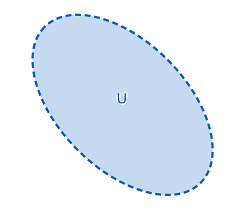
\includegraphics[scale=1.1]{Openset}}
    \caption[Visualising an open set]{\label{fig:Openset}
    An open set formed by the removal of the boundry points of $U$}
\end{figure}

\begin{definition}{Connected Sets}
A set $U\subseteq \mathbb{R}^{2}$ is said to be \textit{connected} if 
\begin{align*}
\forall \, x , y \in U \,,\, \exists \, f \, \vcentcolon [0,1] \to U : f(0) = x \quad \text{and}\quad f(1) = y \quad \text{and} \quad f \,\, \text{continous}.
\end{align*}
that is, if we choose any points in $U$ arbitrarily, there is always some path lying in $U$ joining the points.    
\end{definition}

Let $f\,:\,U \, \to \,  \mathbb{R}^{n}$ where $U$ is an open set in $\mathbb{R}^{2}$, $f$ is said to be $C^{k}$ if $f$ and it's partial derivatives (of order up to k) exist and are continuous. That is $f$ is $C^{k}$ if $f$ is continously differentiable up to order $k$. Furthermore, $f$ is said to be \textit{smooth} if $f$ is  $C^{k} \,\,\, \forall \, k \in \mathbb{N}$. 
\\
\begin{remark}
Recall that if the mixed partial derivatives of a function $f$ are continuous, then they are equal, that is 
\begin{align*}
f_{xy} \, = \, f_{yx}.
\end{align*}
A similar result holds for all higher derivatives. Hence if a function $f$ is \textit{smooth} then it's mixed partial derivatives may be calculated in any order \cite{Shifrin2016}.
\end{remark}

We now state and prove an important Lemma from calculus which we shall use later on

\begin{lemma}\label{lemma:calc}
Suppose $f,\,g\vcentcolon\,(a,\,b)\,\to\,\mathbb{R}$ are differentiable and satisfy $f(t)\cdot g(t)\,=\,const,\,\,\forall t$. Then $f'(t)\cdot g(t)\,=\,-f(t)\cdot g'(t)$. In particular,
\begin{align*}
\lvert\lvert f(t)\rvert\rvert\quad \text{if and only if}\quad  f(t)\cdot f'(t)\,=\,0\quad \text{for all}\,\,\, t.
\end{align*}
\end{lemma}

\begin{proof}
We know a function is constant on some interval if and only if its derivative is everywhere zero, hence from the product rule we have
\begin{align*}
(f\cdot g)'(t)\,=\,f'(t)\cdot g(t)\,+\,f(t)\cdot g'(t).
\end{align*}
so if $f\cdot g$ is constant, then $f\cdot g'\,=\,-f'\cdot g$. In particular, $\lvert \lvert f \rvert\rvert$ is constant if and only if $\lvert \lvert f \rvert\rvert^2\,=\,f\cdot f$ is constant, which occurs if and only if $f\cdot f'\,=\,0$.
\end{proof}

%Need to mention why we want this set to be connected =  So our surface is one piece.
\section{Regular parametizations and surfaces}
We now proceed to the definition of a surface. Informally, we can visualize this as an injective mapping from some open subset of $\mathbb{R}^{2}$ to $\mathbb{R}^{3}$. We will use $(u , v)$ as coordinates in our parameter space, $\mathbb{R}^{2}$, and $(x , y, z) $ as coordinates in our ambient space $\mathbb{R}^{3}$. We note that the subset of $\mathbb{R}^{2}$ is required be open as this naturally introduces the concepts of derivatives to our space. For if a function is defined on an open set then we may easily take the limit at each point. Further a connected set ensures that the surfaces we deal with are also connected, that is, composed of one piece \cite{DC1976}. 

\begin{definition}{}
A \textit{regular paramatization} of a subset $M \, \subset \, \mathbb{R}^{3}$ is a one-to-one function
\begin{align*}
\vect{x} \vcentcolon \, U \, \to \, M \, \subset \, \mathbb{R}^{3} \quad \text{such that} \quad \vect{x_{\bm{u}}} \times \vect{x_{\bm{v}}} \, \neq \, \vect{0}.
\end{align*}
for some open set $U \, \subset \, \mathbb{R}^{2}$. A connected subset $M \, \subset \, \mathbb{R}^{3}$ is called a \textit{surface} if every point in $M$ has some neighbourhood which is regularly parametized. 
\end{definition}

The condition that $\vect{x_{\bm{u}}} \times \vect{x_{\bm{v}}} \, \neq \, \vect{0}$ implies that the vectors $\vect{x_{\bm{u}}} \,\, \text{and} \ \vect{x_{\bm{v}}}$ span a plane. Then the normal vector to the plane spanned by $\vect{x_{\bm{u}}} \,\, \text{and} \ \vect{x_{\bm{v}}}$ is given by $ \vect{x_{\bm{u}}} \times \vect{x_{\bm{v}}}$.

\begin{remark}
The inclusion of the parametization being \textit{regular} in the above definition depends on the condition $\vect{x_{\bm{u}}} \times \vect{x_{\bm{v}}} \, \neq \, \vect{0}$. If the tangent vector fields $\vect{x_{\bm{u}}} \,\,\text{and}\, \,\vect{x_{\bm{v}}}$ are linearly independent at every point in $U$, then it is regular. Clearly if $\vect{x_{\bm{u}}} \,\,\text{and} \,\,\vect{x_{\bm{v}}}$ are linearly independent, then $\vect{x_{\bm{u}}} \times \vect{x_{\bm{v}}} \, \neq \, \vect{0}$, as in the definition.
\end{remark}


\begin{example}\label{ex:232}
We will now look at the parametization of the \textit{torus} and show that it is indeed a regular parametization. It may be parametized by
\begin{align*}
\vect{x}(u,v) = \big((a + b\cos u)\cos v, \,(a + b\cos u)\sin v,\, b\sin u\big), \quad 0 \leq u, v < 2\pi \quad (a>b).
\end{align*}
Then
\begin{align*}
\vect x_u &= (-b\sin u \cos v, \, -b\sin u \sin v, \,b\cos u). \\
\vect x_v &= \big(-(a + b\cos u)\sin v, (a + b\cos u)\cos v,\,0\big).
\end{align*} 
and
\begin{align*}
\vect x_u\times \vect x_v \, = \, -b(a + b\cos u)(\cos u\cos v, \, \cos u\sin v, \, \sin u).
\end{align*}
which is clearly never $\vect{0}$. Hence this is a regular parametization of the torus.
\end{example}

\begin{remark}
We note that the torus is simply a circle rotated about a larger circle lying in an orthogonal plane. This can be readily seen in Fig.~\ref{fig:mytorus} below.
\begin{figure}[H]
    \centerline{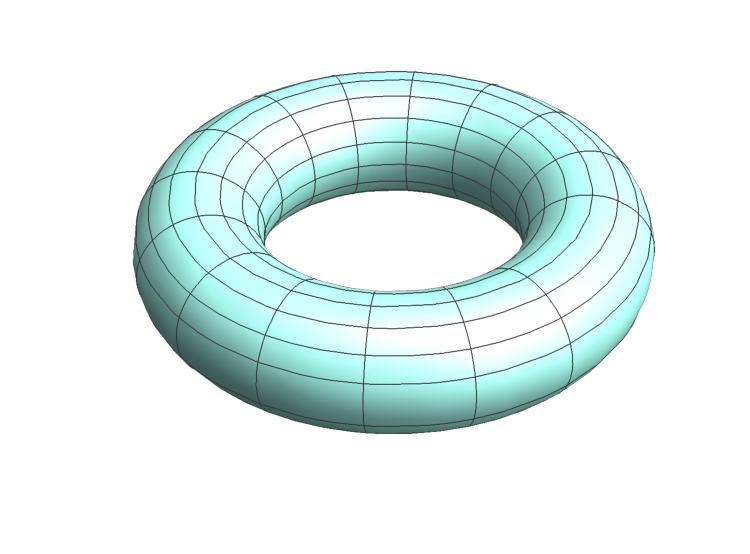
\includegraphics[scale=1]{mytorus}}
    \caption[Parametization of a torus ]{\label{fig:mytorus}
    A torus}
\end{figure}
\end{remark}

The torus is an example of the \textit{surface of revolution}, as we shall see, this too can be regularly parametized. Henceforth we shall be using the general surface of revolution as our example surface.

\begin{example} \label{ex:233}
Let $I \subset \mathbb{R}$ be an interval, and let $\alpha(u) \, = \, \big(0, \,f(u),\,g(u)\big), u \in I$, be a regular parametized plane curve with $f \, > \, 0$. Then the \textit{surface of revolution} formed by a revolution of $\alpha$ about the $z$-axis is parametized by
\begin{align*}
\vect{x}(u,v) \, = \, \big(f(u)\cos v, \,f(u)\sin v, \, g(u)\big), \quad 	u\, \in \, I, \,\, 0\,\leq\,v\,<\,2\pi.
\end{align*}
Then
\begin{align*}
\vect x_u &= \big(f'(u)\cos v,\, f'(u)\sin v, \, g'(u)\big),\\
\vect x_v &= \big(-f(u)\sin v,\, f(u)\cos v, \,0\big).
\end{align*}
and
\begin{align*}
\vect x_u\times \vect x_v \, = \, f(u)\big(-g'(u)\cos v, \, -g'(u)\sin v,\, f'(u)\big).
\end{align*}
which is never zero, and so this is a regular parametization. Fixing $u$ and varying $v$ we generate the \textit{parralels}, which are circles. Fixing $v$ and varying $u$ we generate the \textit{meridians}, which are copies of $\alpha$ rotated an angle of $v$ around the $z$-axis. This can be seen in Figure \ref{fig:SurfaceRev} below.
\end{example}

\begin{figure}[H]
    \centerline{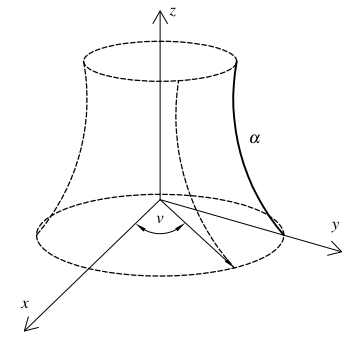
\includegraphics[scale=1]{SurfaceRev}}
    \caption[The Surface Of Revolution]{\label{fig:SurfaceRev}
    The surface of revolution formed by rotating $\alpha$ about the $z$-axis}
\end{figure}

We will now make clear why we desire to work with surfaces with a regular parametization. Recall from calculus that given some differentiable function $f$, the best linear approximation to our function near a point $x = t$ is given by the \textit{tangent line}
\begin{align*}
y \, 	= \, f'(t)(	x \, - \, t) \, + \, f(t).
\end{align*}
Now given some surface, using the same idea above, we would like to make an approximation to our surface at some point. Since we are dealing with a regular parametized surface we know that the tangent vector fields $\vect x_u \,\, \text{and}\, \, \vect x_v$ span a plane, and since both $\vect x_u \,\, \text{and} \,\, \vect x_v$ are tangent to $\vect{x}(u,v)$ at all points, the plane spanned by $\vect x_u \,\, \text{and} \,\, \vect x_v$ is the \textit{tangent plane}.

\begin{definition}{}
Let $x \vcentcolon U \, \to \, M \, \subset \, \mathbb{R}^{3}$ be a regular parametization of a surface $M$. Let $P \, \in \, M$ with $P$ = $\vect{x}(u_0,v_0)$. The \textit{tangent plane} of $M$ at point $P$ is defined as the subspace $T_PM$ spanned by $\vect x_u \,\, \text{and} \,\, \vect x_v$, evaluated at $P$. That is 
\begin{align*}
T_PM \coloneqq \{\alpha \vect x_u (u_0,v_0) \, + \, \beta \vect x_v(u_0,v_0)\, |\, \alpha,\beta \, \in \mathbb{R}\}.
\end{align*}
\end{definition}

Now since the parametization is regular we know $\vect x_u \times \vect x_v$ exists and is orthogonal to $T_PM$. We now define the \textit{unit normal} of the surface to be 
\begin{align*}
\vect{n} \, = \, \dfrac{\vect x_u \times \vect x_v}{\lvert\lvert\vect x_u \times \vect x_v\rvert\rvert}
\end{align*}

\begin{figure}[H]
    \centerline{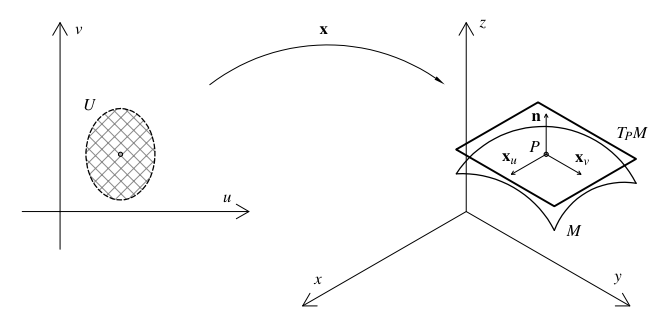
\includegraphics[scale=1]{TangentPlane}}
    \caption[The Tangent Plane]{\label{fig:TangentPlane}
    The tangent plane spanned by $\vect x_u \,\, \text{and} \,\, \vect x_v$, adapted from \cite{Shifrin2016}}
\end{figure}

The geometry of some space curve is best understood when parametized by arclength, that is, if $\alpha(u)$ is a curve parametized by arclength, then $\lvert\lvert\alpha'(u)\rvert\rvert \, = \, 1$. To extend this understanding to three-dimensional surfaces (and higher dimensions too), we wish to find a parametization  $\vect{x}(u,v)$ of a surface such that the tangent vector fields form an orthonormal basis at each point \cite{Shifrin2016}. That is, $\{\vect x_u,\vect x_v\}$ forms a basis with $ \vect x_u\, \text{and} \, \vect x_v$ unit. Such parametizations lead us to define the \textit{First Fundamental Form}, a quadratic form on $T_PM$. As we shall see, the importance of the First Fundamental Form is central in dealing with metric properties of a surface.
\clearpage
\chapter{The First Fundamental Form}
\section{Introduction}
Formally, the first fundamental form is the inner product of the tangent vectors on a surface in three-dimensional Euclidean space. It is induced canonically from the usual dot product of $\mathbb{R}^3$. The first fundamental form fully describes the metric properties of a surface, this allows one to make calculations based upon areas or lengths of curves in a manner consistent with the ambient space. This is particularly important as it allows us, for example, to find the length of a curve on a surface without needing any knowledge of the embedding of said surface. 
\section{The First Fundamental Form}
\begin{definition}{The First Fundamental Form}
Let $M$ be a regular surface with $\vect{U}, \, \vect{V} \, \in \, T_PM$. Then the \textit{First Fundamental Form} is defined to be
\begin{align*}
\RN{1}_P(\vect{U}, \, \vect{V}) \, = \,  \vect{U} \cdot \vect{V}.
\end{align*}
Since $M$ is regular, we have the natural basis $\{\vect x_u,\vect x_v\}$ and so we could represent $\vect{U} \, \text{and} \, \vect{V}$ in terms of this basis. This leads us to define
\begin{align*}
E \, &= \, \RN{1}_P(\vect x_u,\vect x_u) \, = \, \vect x_u \cdot \vect x_u,\\
F \, &= \, \RN{1}_P(\vect x_u,\vect x_v) \, = \, \vect x_u \cdot \vect x_v \, = \, \vect x_v \cdot \vect x_u \, = \, \RN{1}_P(\vect x_v,\vect x_u),\\
G \, &= \, \RN{1}_P(\vect x_v,\vect x_v) \, = \, \vect x_v \cdot \vect x_v.
\end{align*}
Now if $\vect{U} \ = \, a\vect x_u \, + \, b\vect x_v \, \text{and} \,\, \vect{V} \,\, = \, c\vect x_u \, + \, d\vect x_v \, \in T_PM$, then we have
\begin{align*}
\vect{U} \cdot \vect{V} \, = \, \RN{1}_P(\vect{U},\, \vect{V}) \, = \, (a\vect x_u \, + \, b\vect x_v)\cdot(c\vect x_u \, + \, d\vect x_v) \, = \, E(ac) \, + \, F(ad \, + \, bc) \, + \, G(bd).
\end{align*}
We can conveniently view this as a symmetric matrix as follows
\begin{align*}
\vect{U} \cdot \vect{V} \, = \,
\begin{bmatrix}
    a\vect x_u \\
    b\vect x_v
\end{bmatrix}
\cdot
\begin{bmatrix}
    c\vect x_u & d\vect x_v
\end{bmatrix}
\, = \,
\begin{bmatrix}
    ac\vect x_u\cdot\vect x_u & ad\vect x_u\cdot\vect x_v\\
    bc\vect x_v\cdot\vect x_u & bd\vect x_v\cdot\vect x_v
\end{bmatrix}
\, = \,
 \begin{bmatrix}
    a\\
    b
\end{bmatrix}^\intercal
\begin{bmatrix}
    E & F\\
    F & G
\end{bmatrix}
\begin{bmatrix}
    c\\
    d
\end{bmatrix}.
\end{align*}
That is
\begin{align*}
\RN{1}_P \, = \,
\begin{bmatrix}
    E & F\\
    F & G
\end{bmatrix}.
\end{align*}
We note that the first fundamental form of one argument is simply the inner product of that particular vector with itself, satisfying
\begin{align*}
\RN{1}_P(\vect{U},\,\vect{U}) \, = \, \lvert\lvert\vect{U}\rvert\rvert^2 \, = \, Ea^2 \, +\, 2Fab \, +\, Gb^2.
\end{align*}
\end{definition}

\section{The Intrinsic Properties}
We shall now consider a curve lying in our surface $M$. Working with the regular parametization $\vect{x} \vcentcolon U \, \to \, M \, \subset \, \mathbb{R}^{3}$, if $\alpha \, \vcentcolon \, I \, \to \mathbb{R}^{3}$ is a curve contained in our surface, then the open interval $I$ must be such that:
\begin{align*}
\alpha(t) \, \in \, \vect{x}(U) \, = \, \{\vect{x}(u,v) \, : \, (u,v)\, \in \, U\} \quad \forall \, t \, \in \, I.
\end{align*}
That is, for each $t \, \in \, I$, there exists $\big(u(t),v(t)\big) \, \in \, U$ such that $\alpha(t) \, = \, \vect{x}\big(u(t),v(t)\big)$. Hence we may consider any such curve as a map of the form:
\begin{align*}
\vect{x} \circ (u,v) \, \vcentcolon \, t \, \mapsto \, \vect{x}\big(u(t),v(t)\big).
\end{align*}
where
\begin{align*}
(u,v) \, \vcentcolon \, I \, \to \, U \quad \text{by} \quad t \, \mapsto \, \big(u(t),v(t)\big).
\end{align*}

Now if $\alpha(t)$ is a curve lying on our surface, then by the chain rule we have that
\begin{align*}
\vect{\alpha}'(t) \, = \, \deriv{\vect{\alpha}}{t} \, = \, \deriv{\vect{\alpha}}{u} \cdot \deriv{u}{t} \, + \, \deriv{\vect{\alpha}}{v} \cdot \deriv{v}{t} \, = \, \vect{x_{\bm{u}}}\cdot u'(t) \, + \, \vect{x_{\bm{v}}}\cdot v'(t).
\end{align*}
which gives us 
\begin{align*}
\vect{\alpha}'(t) \cdot \vect{\alpha}'(t) \, &= \, \vect x_u\cdot\vect x_u(u')^2 \,+ \,\vect x_u\cdot\vect x_vu'v' \,+\, \vect x_v\cdot\vect x_uv'u' \, + \,\vect x_v\cdot\vect x_v(v')^2\\
&= \,E(u')^2 \, + \, 2Fu'v' \, + \, G(v')^2\\
&= \RN{1}_{\vect{\alpha}(t)}\big(\vect{\alpha}'(t)\, , \, \vect{\alpha}'(t)\big).
\end{align*}
Then if $\alpha(t)$ is given along an interval $I$ = (a,b). We can calculate the length of our curve by the usual formula


\begin{align*}
length(\vect{\alpha}) \, &= \, \int_a^b \lvert \vect{\alpha}(t)\rvert  \, dt\\
&= \int_a^b \sqrt{\RN{1}_{\vect{\alpha}(t)}\big(\vect{\alpha}'(t)\, , \, \vect{\alpha}'(t)\big)}  \, dt\\
&= \int_a^b \sqrt{E\big(u(t),v(t))(u'(t)\big)^2 \, + \, 2F\big(u(t),v(t)\big)u'(t)v'(t) \, + \, G\big(u(t),v(t))(v'(t)\big)^2} \, dt.\\
\end{align*}


Recall from calculus that $ds$ is an infinitesimal piece of arc length, we can then express the square of the \textit{line element} as
\begin{align*}
ds^2 \, &= \, \lvert d \vect{\alpha} \rvert^2 \, = \, d \vect{\alpha}\cdot d \vect{\alpha} \\
&=\,  (\vect x_udu \, + \, \vect x_vdv) \cdot (\vect x_udu \, + \, \vect x_vdv)\\
&= \, Edu^2 \, + \, 2Fdudv \, + \, Gdv^2.
\end{align*} 
Then solving for \textit{s} (arc length) by integration gives us
\begin{align*}
s \, = \, \int \, ds \, = \, \int \sqrt{Edu^2 \, + \, 2Fdudv \, + \, Gdv^2}.
\end{align*}
However, based on the discussion above, if this curve is lying in our surface, it can be expressed as a function of a single parameter $t$ and we have 
\begin{align*}
s(t) \, = \, \int \, ds \, = \, \int \sqrt{E(u')^2 \, + \, 2Fu'v' \, + \, G(v')^2}dt.
\end{align*}

\begin{remark}
What we have developed here is a method of measuring a curve which lies in our surface using nothing more than the tangential components at each point on the curve! If we imagine some denizen on our surface capable of only conceiving the 2-dimensional space, he would be able to measure a curve accurately without needing any knowledge of the third dimension \cite{Shifrin2016}. This makes length of a curve an \textit{intrinsic} property of the surface, that is, a property  which depends only on the surface itself and not how it is embedded in the ambient space. We shall see later on certain properties require reference to the embedding of the surface. 
\end{remark}

\begin{example}
Consider the general surface of revolution, seen in Example \ref{ex:233}. As we saw, it's regular parametization is given by
\begin{align*}
\vect{x}(u,v) \, = \, \big(f(u)\cos v, \,f(u)\sin v, \, g(u)\big), \quad 	u\, \in \, I, \,\, 0\,\leq\,v\,<\,2\pi.
\end{align*}
Then we found 
\begin{align*}
\vect x_u &= \big(f'(u)\cos v,\, f'(u)\sin v, \, g'(u)\big), &
\vect x_v &= \big(-f(u)\sin v,\, f(u)\cos v, \,0\big).\\
\end{align*}
and so we have
\begin{align*}
E \,=\,\vect x_u\cdot\vect x_u \, &= \, f'(u)^2(\cos^2v\,+\,\sin^2v)\,+\,g'(u)^2\\
&=\,f'(u)^2\,+\,g'(u)^2,\\\\
F\,=\,\vect x_u\cdot\vect x_v \, &= \, -f(u)f'(u)\cos v\sin v \, +\, f(u)f'(u)\cos v\sin v\\
&=\,0,\\\\
G\,=\,\vect x_v\cdot\vect x_v\, &=\,f(u)^2\sin^2v\,+\,f(u)^2\cos^2v\\
&=\,f(u)^2.
\end{align*}
We can then consider a regularly parametized curve on our surface by fixing $u$ and varying $v$, as seen in Figure \ref{fig:SurfaceRevCurve}. That is, our curve has form
\begin{align*}
\alpha(t)\,=\,\vect{x}(u(t_0),v(t)) \quad t_0 \,\in\,I,\,\, 0\,\leq\,t\,<\,2\pi.
\end{align*}

\begin{figure}[H]
    \centerline{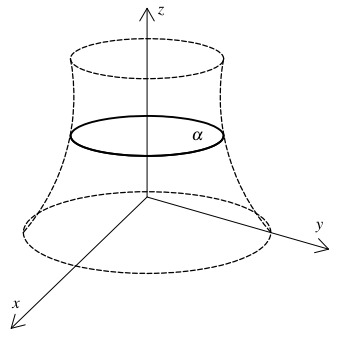
\includegraphics[scale=1]{SurfaceRevCurve}}
    \caption[A Curve on the Surface of Revolution]{\label{fig:SurfaceRevCurve}
    The curve $\alpha$ formed by fixing $u$ and varying $v$.}
\end{figure}

Using the above coefficients, we can solve for the length of the curve
\begin{align*}
length(\alpha)\,=\,\int_0^{2\pi}\,\sqrt{E\big(u(t_0),v(t)\big)\big(u'(t_0)\big)^2 \, + \, 2F\big(u(t_0),v(t)\big)u'(t_0)v'(t) \, + \, G\big(u(t_0),v(t)\big)\big(v'(t)\big)^2}dt.
\end{align*}
but since u is fixed and v(t) = t
\begin{align*}
u'(t_0)\,=\,0 \quad and \quad v'(t)\,=\,1.
\end{align*}
we have
\begin{align*}
length(\alpha)\,&=\,\int_0^{2\pi}\,\sqrt{\Big(f'(u(t_0)^2\,+\,g'\big(u(t_0)\big)^2\Big)\cdot \big(u'(t_0)\big)^2\,+\,2(0)u'(t_0)v'(t)\,+\,f\big(u(t_0))^2(v'(t)\big)^2}\\
&=\,\int_0^{2\pi}\,\sqrt{f\big(u(t_0)\big)^2}dt\\
&=\, f\big(u(t_0)\big)\int_0^{2\pi}dt\\
&=\, 2\pi f\big(u(t_0)\big).
\end{align*}
This result is expected, as the curve we are considering is simply a circle of radius $f(u(t_0))$ traced along our surface of revolution.\\
\end{example}
Recall from calculus that the angle $\theta$ between two vectors $\vect{a},\,\vect{b}$ is such that
\begin{align*}
\cos \theta \,=\,\dfrac{\vect{a}\cdot\vect{b}}{\lvert\lvert\vect{a}\rvert\rvert\cdot\lvert\lvert\vect{b}\rvert\rvert}.
\end{align*}
Then if $\alpha(t)\,=\,\vect{x}(u_1(t),v_1(t))$ and $\beta(t)\,=\,\vect{x}(u_2(t),v_2(t))$  are two regularly parametized curves on our surface intersecting at some point $t\,=\,t_0$, then their angle of intersection is given by
\begin{align*}
\cos \theta \,=\,\dfrac{\alpha'(t_0) \cdot \beta'(t_0)}{\lvert\lvert\alpha'(t_0)\rvert\rvert \cdot \lvert\lvert\beta'(t_0)\rvert\rvert}\,=\,Eu_1'v_1'\,+\,F(u_1'v_2'\,+\,u_2'v_1')\,+\,Gv_1'v_2'.
\end{align*}
Further, the angle between the coordinate curves of a parametization $\vect{x}(u,v)$ is 
\begin{align*}
\cos \theta \, = \, \dfrac{\vect x_u\cdot\vect x_v}{\lvert\lvert\vect x_u\rvert\rvert\cdot\lvert\lvert\vect x_v\rvert\rvert}\,=\,\dfrac{F}{\sqrt{EG}}.
\end{align*}

From this we see that two tangent vectors $\alpha'(t)\,\text{and}\,\beta'(t)$ are orthogonal if and only if $Eu_1'v_1'\,+\,F(u_1'v_2'\,+\,u_2'v_1')\,+\,Gv_1'v_2' = 0$. Furthermore coordinate curves of a parametization are orthogonal if and only if $F(u,v) \,= \,0$. We note that when calculating the angle, again, only the tangential components to our surface are needed.

\begin{definition}{Conformal Parametizations}
A parametization $\vect{x}(u,v)$ is \textit{conformal} if angles measured in our coordinate space agree with corresponding angles in our tangent space, $T_PM$, for all $P$.
\end{definition}

\begin{prop}
A parametization $\vect{x}(u,v)$ is conformal if and only if $E\,=\,G$ and $F\,=\,0$.
\end{prop}

\begin{proof}
Let $\vect x(u,v)$ be a conformal parametization. Consider the vectors $\vect e_1$ and $\vect e_2$ in $\mathbb{R}^2$ with $\vect e_1$ orthogonal to $\vect e_2$.

Clearly the corresponding vectors in the tangent plane are $\vect x_u$ and $\vect x_v$ respectively, with $\vect x_u$ orthogonal to $\vect x_v$. Then, by our assumption,
\begin{align*}
\cos\theta\,=\,\dfrac{\vect e_1\cdot\vect e_2}{\lvert\lvert\vect e_1\rvert\rvert\cdot\lvert\lvert\vect e_2\rvert\rvert}\,=\,\dfrac{\vect x_u\cdot\vect x_v}{\lvert\lvert\vect x_u\rvert\rvert\cdot\lvert\lvert\vect x_v\rvert\rvert}\,=\,\dfrac{F}{\sqrt{EG}}
\end{align*}
but $\vect e_1\cdot\vect e_2\,=\,0\,\Longrightarrow\,F\,=\,0$.

Now $(\vect e_1\,-\,\vect e_2)$ and $(\vect e_1\,+\,\vect e_2)$ are also orthogonal to one another. The corresponding vectors in the tangent plane are $(\vect x_u\,-\,\vect x_v)$ and $(\vect x_u\,+\,\vect x_v)$ respectively. Then, by our assumption,
\begin{align*}
\cos\theta\,=\,\dfrac{(\vect e_1\,-\,\vect e_2)\cdot(\vect e_1\,+\,\vect e_2)}{\lvert\lvert\vect e_1\,-\,\vect e_2\rvert\rvert\cdot\lvert\lvert\vect e_1\,+\,\vect e_2\rvert\rvert}\,=\,\dfrac{(\vect x_u\,-\,\vect x_v)\cdot(\vect x_u\,+\,\vect x_v)}{\lvert\lvert\vect x_u\,-\,\vect x_v\rvert\rvert\cdot\lvert\lvert\vect x_u\,+\,\vect x_v\rvert\rvert}\,=\,\dfrac{E\,-\,G}{E\,+\,G}
\end{align*}
but $(\vect e_1 \,-\,\vect e_2)\cdot(\vect e_1 \,+\,\vect e_2)\,=\,0\,\Longrightarrow\,E\,-\,G\,=\,0\,\Longrightarrow\,E\,=\,G$ as required.
$\\$Conversely, suppose that $E\,=\,G$ and $F\,=\,0$. Let
\begin{align*}
\vect w\,&=\,(a,b)\,\in\,\mathbb{R}^2\quad\text{corresponding to}\quad \vect w_m\,=\,a\vect x_u\,+\,b\vect x_v\,\in\,T_PM,\\
\vect z\,&=\,(c,d)\,\in\,\mathbb{R}^2\quad\text{corresponding to}\quad \vect z_m\,=\,c\vect x_u\,+\,d\vect x_v\,\in\,T_PM.\\
\end{align*}
So we have,
\begin{align*}
&\RN{1}_P(\vect w_m,\vect z_m)\,=\,acE\,+\,F(ad\,+\,bc)\,+\,Gbd\,=\,E(ac\,+\,bd)\,=\,E(\vect w\cdot \vect z),\\
&\RN{1}_P(\vect w_m,\vect w_m)\,=\,E(\vect w\cdot \vect w),\\
&\RN{1}_P(\vect z_m,\vect z_m)\,=\,E(\vect z\cdot \vect z).
\end{align*}
Then
\begin{align*}
\dfrac{\RN{1}_P(\vect w_m,\vect z_m}{\sqrt{\RN{1}_P(\vect w_m,\vect w_m)\RN{1}_P(\vect z_m,\vect z_m)}}\,=\,\dfrac{E(\vect w\cdot \vect z}{\sqrt{E^2(\vect w\cdot \vect w)(\vect z\cdot \vect z)}}\,=\,\dfrac{\vect w\cdot\vect z}{\lvert\lvert\vect w\rvert\rvert\lvert\lvert\vect z\rvert\rvert}.
\end{align*}
Hence the parametization is conformal.
\end{proof}


We now turn our attention to the area of the surface. It will be shown that we can calculate the area of some bounded region on a regular surface $M$. A regular \textit{domain} of M is an open and connected subset of $M$ such that its boundary is the image of a disk by some differentiable homeomorphism which is regular except at a finite number of points \cite{DC1976}. A $region$ of $M$ is the union of the domain and its boundary. We say a region of $M \, \subset \, \mathbb{R}^3$ is \textit{bounded} if it is contained in some ball of $\mathbb{R}^3$
$\\$
\begin{prop}
Let M be a regular surface, there exists a function $\lambda\,\neq\,0$ such that
\begin{align*}
E\cdot G\,-\,F^2\,=\,\lambda^2.
\end{align*}
\end{prop}

\begin{proof}
Since
\begin{align*}
\begin{bmatrix}
    E & F\\
    F & G
\end{bmatrix}
\,=\,
\begin{bmatrix}
    \vect x_u\cdot\vect x_u & \vect x_u\cdot\vect x_v\\
    \vect x_u\cdot\vect x_v & \vect x_v\cdot\vect x_v
\end{bmatrix}
\,=\,
\begin{bmatrix}
    | & |\\
    \vect x_u & \vect x_v\\
    | & |
\end{bmatrix}^\intercal
\begin{bmatrix}
    | & |\\
    \vect x_u & \vect x_v\\
    | & |
\end{bmatrix}.
\end{align*}
taking determinant of both sides give
\begin{align*}
EG\,-\,F^2\,&=\,\det\begin{pmatrix}
\begin{bmatrix}
    \vect x_u\cdot\vect x_u & \vect x_u\cdot\vect x_v\\
    \vect x_u\cdot\vect x_v & \vect x_v\cdot\vect x_v
\end{bmatrix}
\end{pmatrix}
\,	=\,
\det\begin{pmatrix}
\begin{bmatrix}
    \vect x_u\cdot\vect x_u & \vect x_u\cdot\vect x_v & 0\\
    \vect x_u\cdot\vect x_v & \vect x_v\cdot\vect x_v & 0\\
     0 & 0 & 1
\end{bmatrix}
\end{pmatrix}\\
&=\,
\det\begin{pmatrix}
\begin{bmatrix}
    | & | & |\\
    \vect x_u & \vect x_v & \vect{n}\\
    | & | & |\\
\end{bmatrix}^\intercal
\begin{bmatrix}
    | & | & |\\
    \vect x_u & \vect x_v & \vect{n}\\
    | & | & |\\
\end{bmatrix}
\end{pmatrix}
\,=\,
\begin{pmatrix}\det
\begin{bmatrix}
    | & | & |\\
    \vect x_u & \vect x_v & \vect{n}\\
    | & | & |\\
\end{bmatrix}
\end{pmatrix}^2.
\end{align*}
Which is the square of the volume of the parallelepiped spanned by $\vect x_u,\, \vect x_v\, \,\text{and}\,\, \vect{n}$. However $\vect{n}$ is a unit vector orthogonal to the plane spanned by $\vect x_u\,\text{and}\,\vect x_v$. So we have the square of the area of the parrallelogram spanned by $\vect x_u\,\,\text{and}\,\,\vect x_v$. That is
\begin{align*}
EG\,-\,F^2\,=\,\lvert\lvert\vect x_u\,\times\,\vect x_v\rvert\rvert^2 \,>\,0.
\end{align*}
\end{proof}

Let us consider a parralelogram with vertices $\vect{x}(u,v),\,\vect{x}(u\,+\,du,v),\,\vect{x}(u\,+\,du,v\,+\,dv),\,\vect{x}(u,v\,+\,dv)$. As seen in Figure \ref{fig:AreaParm}, the area may be approximated by
\begin{align*}
dA\,=\,\lvert\lvert\vect x_udu\,\times\,\vect x_vdv\rvert\rvert.
\end{align*}
Which implies the surface area is
\begin{align*}
A\,=\,\int\int_U\,\lvert\lvert\vect x_u\,\times\,\vect x_v\rvert\rvert dudv\,=\,\int\int_U\,\sqrt{EG\,-\,F^2} dudv.
\end{align*}

\begin{figure}[H]
    \centerline{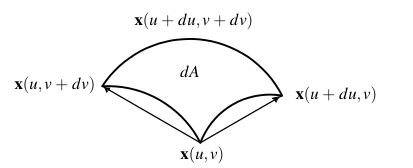
\includegraphics[scale=1]{AreaParm}}
    \caption[Approximating the Area of an Infinitesimal Parallelogram]{\label{fig:AreaParm}
    The Area of an Infinitesimal Parallelogram, adapted from \cite{MIT}}
\end{figure}

\begin{example}
We return again to the general surface of revolution from Example \ref{ex:233}. We now seek to calculate the area spanned by the surface. Recall
\begin{align*}
E\,=\,f'(u)^2\,+\,g'(u)^2, \quad F\,=\,0,\quad G\,=\,f(u)^2.
\end{align*}

and so if $u\,\in\,I\,=\,[a,b]$ and $0\,\leq\,v\,<\,2\pi$

\begin{align*}
A\,=\,\int\int_U\,\sqrt{EG\,-\,F^2}dudv\,&=\,\int_0^{2\pi}\int_a^b\, \sqrt{\big(f'(u)^2\,+\,g'(u)^2\big)\cdot f(u)^2}dudv\\
&=\,2\pi\int_a^b\lvert f(u) \rvert \sqrt{\big(f'(u)^2\,+\,g'(u)^2\big)}du.\\
\end{align*}

To verify this result is consistent with what we know, let us take the specific case of the torus from Example \ref{ex:232}. Then since
\begin{align*}
f(u)\,=\,(a\,+\,b\cos u)\quad \text{and} \quad g(u)\,=\,b\sin u.
\end{align*}
we have
\begin{align*}
f'(u)\,=\,-b\sin u\quad \text{and} \quad g'(u)\,=\,b\cos u.
\end{align*}
so
\begin{align*}
f'(u)^2\,+\,g'(u)^2\,&=\,b^2\sin^2u\,+\,b^2\cos^2u\\
&=\,b^2.
\end{align*}
Subbing this result into our above equation gives
\begin{align*}
A\,&=2\pi\int_a^b\lvert f(u) \rvert \sqrt{\big(f'(u)^2\,+\,g'(u)^2\big)}du\\
&=\,2\pi\int_0^{2\pi}(a\,+\,b\cos u)\sqrt{b^2}\,du\\
&=\,2\pi b\bigg[\int_0^{2\pi} a\,du \,+\,\int_0^{2\pi}b\cos u\,du\bigg]\\
&=\,2\pi b\bigg[a\int_0^{2\pi}du \,+\,b\int_0^{2\pi}\cos u\,du\bigg]\\
&=\,2\pi b\bigg[a\left. u \right|_0^{2\pi}\,+\,b\left.\sin u \right|_0^{2\pi}\bigg]\\
&=\,2\pi b [2\pi a]\\
&=\, 4\pi^2 a b.\\
\end{align*}
Which is indeed the surface area of the torus.
\end{example}

In the above discussions, we have always taken some regular parametizaion of our surface, one may be wondering, if we took two different parametizations of our surface $M$ do we obtain the same results? Indeed we do, as we shall show for the area calculation. For this we will need to call upon the concept of change of parameters.
$\\$
\begin{prop}
Let $P$ be a point on a regular surface $M$ and let $\vect x \vcentcolon \,U\,\subset\,\mathbb{R}^2\,\to\,M,\,\vect x^*\vcentcolon\,U^*\,\to\,M$ be two parametizations of M such that $P\,\in\,\vect x(U)\,\cap\,\vect x^*(U^*)\,=\,V$. Then the \textit{change of parameters} $h\,=\,\vect x^{-1}\circ\vect x^*\vcentcolon \vect x^{*\,-1}(V)\,\to\,\vect x^{-1}(V)$ (\ref{fig:ChangeOfParamSS}) is a \textit{diffeomorphism}, that is $h$ is differentiable and has a differentiable inverse $h^{-1}$.
\end{prop}

\begin{figure}[H]
    \centerline{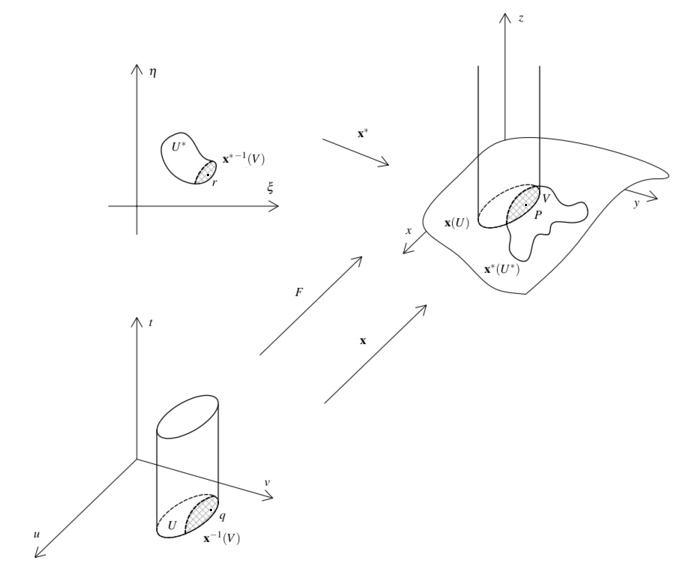
\includegraphics[scale=1]{ChangeOfParamSS}}
    \caption[The Change of Parameters]{\label{fig:ChangeOfParamSS}
    The Change of Parameters, adapted from \cite{DC1976}}
\end{figure}

\begin{proof}
$h\,=\,\vect x^{-1}\circ\vect x^*$ is a homeomorphism (A bijective function which is continuous and has continuous a inverse) since it is composed of homeomorphisms. Let $r\,\in\,\vect x^{*\,-1}(V)$ and set $q\,=\,h(r)$.

Since $\vect x(u,v)\,=\,\big(x(u,v),\,y(u,v)\,,z(u,v)\big)$ is a parametization, we can assume (by renaming the axis if necessary) that
\begin{align*}
\dfrac{\partial (x,y)}{\partial (u,v)}(q)\,\neq\,0.
\end{align*}
We extend $\vect x$ to the map $F\vcentcolon\,U\,\times\,\mathbb{R}\to\mathbb{R}^3$ defined by 
\begin{align*}
F(u,\,v,\,t)\,=\,\big(x(u,v),\,y(u,v),\,z(u,v)\,+\,t\big),\quad (u,v)\,\in\,U,\,t\,\in\,\mathbb{R}.
\end{align*}
Geometrically, $F$ maps a vertical cylinder $C$ over $U$ onto a "vertical cylinder" over $\vect x(U)$ by mapping each section of $C$ with height $t$ into the surface $\vect x(u,v)\,+\,te_3$, where $e_3$ is the unit vector over the $z$ axis. Clearly $F$ is differentiable and that the restriction $\left. F \right| U\,\times\,\{0\}\,=\,\vect x$.

We now find the determinant of the differential $dF_q$
\begin{align*}
\det dF_q = \begin{vmatrix}
    \dfrac{\partial x}{\partial u} & \dfrac{\partial x}{\partial v}	& 0\\
    \dfrac{\partial y}{\partial u} & \dfrac{\partial y}{\partial v} & 0 \\
    \dfrac{\partial z}{\partial u} & \dfrac{\partial z}{\partial v} & 1
\end{vmatrix}\,=\,\dfrac{\partial (x,y)}{\partial (u,v)}(q)\,\neq\,0.
\end{align*}
We may then apply the inverse function theorem, which guarantees the existence of some neighbourhood $Q$ of $\vect x(q)$ in $\mathbb{R}^3$ such that $F^{-1}$ exists and is differentiable in $Q$.

By continuity of $\vect x^*$, there exists a neighbourhood $R$ of $r$ in $U^*$ such that $\vect x^*(R)\,\subset\,Q$. Notice that $\left. h \right| R\,=\,F^{-1}\circ\left.\vect x^*\right| R$ is a composition of differentiable maps. Thus, applying the chain rule, we see that $h$ is differentiable at $r$. Since $r$ is arbitrary, $h$ is differentiable on $\vect x^*(V)$.

Similarily the map $h^{-1}$ is differentiable, and so $h$ is a diffeomorphism.
\end{proof}

That is, if $\vect x(u,v)\,=\,\big(x(u,v),\,y(u,v),\,z(u,v)\big)$ and $\vect x^*(\xi,\eta)\,=\,\big(x(\xi,\eta),\,y(\xi,\eta),\,z(\xi,\eta)\big)$ where $(u,v)\,\in\,U$ and $(\xi,\eta)\,\in\,U^*$. Then the change of cooridnates $h$, given by

\begin{align*}
u\,=\,u(\xi,\eta),\quad v\,=\,v(\xi,\eta),\quad (\xi,\eta)\,\in\,\vect x^{*\,-1}(V).
\end{align*}
has the property that $u$ and $v$ have continuous partial derivatives of all orders, and the map $h$ has inverse, giving
\begin{align*}
\xi\,=\,\xi(u,v),\quad\eta\,=\,\eta(u,v),\quad (u,v)\,\in\,\vect x^{-1}(V).
\end{align*}
where $\xi$ and $\eta$ also have continuous partial derivatives of all orders. Since
\begin{align*}
\dfrac{\partial(u,v)}{\partial(\xi,\eta)}\cdot\dfrac{\partial(\xi,\eta)}{\partial(u,v)}\,=\,1.
\end{align*}
implying that the determinants of the Jacobian of both $h$ and $h^{-1}$ are nonzero everywhere \cite{DC1976}.
$\\$
\begin{remark}
We require the determinant of the Jacobian to be nonzero everywhere as such functions have important properties such as mapping open balls to open balls. Further, such functions are said to be open maps, that is, they map open sets to open sets \cite{Mathonline}. This is obviously important when undergoing a change of coordinates, for if a patch on the surface is open under parametization $\vect x$ then we obviously expect it to be open under $\vect x^*$. Since the Jacobian determinants of our change of coordinates, $h$ and $h^{-1}$, is nonzero everywhere, this is indeed the case.
\end{remark}

\begin{prop}
Let $M$ be a regular surface, the equation
\begin{align*}
A\,=\,\int\int_U\,\lvert\lvert\vect x_u\,\times\,\vect x_v\rvert\rvert dudv.
\end{align*}
is independent of the parametization $\vect{x}(u,v)$.
\end{prop}
\begin{proof}
Let $\vect{x}^*(u^*,v^*)\,\vcentcolon\,U^*\,\to\,M$ be another parametization of our surface $M$. Let $\partial(u,v)/\partial(u^*,v^*)$ be the Jacobian of the change of parameteres $h\,=\,\vect{x}^{-1}\circ\vect{x}^*$. Then 
\begin{align*}
\int\int_{U^*}\,\lvert\lvert\vect x_u^*\,\times\,\vect x_v^*\rvert\rvert du^*dv^*\,&=\,\int\int_{U^*}\lvert\lvert\vect x_u\,\times\,\vect x_v\rvert\rvert \lvert \dfrac{\partial(u,v)}{\partial(u^*,v^*)} \rvert du^*dv^*\\
&=\int\int_{U}\,\lvert\lvert\vect x_u\,\times\,\vect x_v\rvert\rvert dudv.
\end{align*}
where the last equality comes from the theorem of change of variables in multivariable calculus. Hence independence is proved.
\end{proof}

\begin{remark}
This independence is of course expected. If the integral was dependent on the parametization of $M$, then two different local parametizations of $M$ around some point $P$ would result in two different areas being found. Obviously we cannot have two different areas for the same region.
\end{remark}

Suppose we have two surfaces $M$ and $M^*$, they are said to be \textit{isometric} if metrically they behave the same. That is there is a one-to-one correspondence between their points under which a rectifiable (finite length) curve in $M$ corresponds to a rectifiable curve of equal length in $M^*$ \cite{DC1976}. More formally

\begin{definition}{Isometric Surfaces}
Surfaces $M$ and $M^*$ are \textit{locally isometric} if for each $P\,\in\,M$ there exists regular parametizations $\vect{x}\,\vcentcolon\,U\,\to\,M$ and $\vect{x}^*\,\vcentcolon\,U\,\to\,M^*$ such that $\RN{1}_P\,=\,\RN{1}^*_{P^*}$ whenever $P\,=\,\vect{x}(u,v)$ and $P^*\,=\,\vect{x}^*(u,v)$.
\end{definition}

\begin{remark}
From the above it is intuitively clear that the plane is locally isometric to the cylinder \cite{Shifrin2016}. If we cut the cylinder along one of its rulings we could easily unroll it onto part of a plane. The mentioned corresepondence between two equal length curves implies that a local isometry is distance preserving. This can easily be seen below
\end{remark}

\begin{prop}
Let $M$ and $M^*$ be a locally isometric surfaces. If $\alpha\,\subset\,\,M$ and $\alpha^*\,\subset\,M^*$ are corresponding paths, then $length(\alpha)\,=\,length(\alpha^*)$
\end{prop}
\begin{proof}
Suppose $\alpha\,\subset\,\,M$ and $\alpha^*\,\subset\,M^*$ are corresponding paths defined along $[a,b]$. Then 
\begin{align*}
length(\alpha)\,&=\, \int_a^b \sqrt{\RN{1}_{\vect{\alpha}(t)}(\vect{\alpha}'(t)\, , \, \vect{\alpha}'(t))}  \, dt\\
&= \int_a^b \sqrt{E(u(t),v(t))(u'(t))^2 \, + \, 2F(u(t),v(t))u'(t)v'(t) \, + \, G(u(t),v(t))(v'(t))^2} \, dt,\\
\text{and}&\\
length(\alpha^*)\,&=\, \int_a^b \sqrt{\RN{1}_{\vect{\alpha^*}(t)}(\vect{\alpha^*}'(t)\, , \, \vect{\alpha^*}'(t))}  \, dt\\
&= \int_a^b \sqrt{E^{*}(u(t),v(t))(u'(t))^2 \, + \, 2F^*(u(t),v(t))u'(t)v'(t) \, + \, G^*(u(t),v(t))(v'(t))^2} \, dt.
\end{align*}
But since $M$ and $M^*$ are locally isometric, we have $\RN{1}_P\,=\,\RN{1}^*_{P^*}$. That is
\begin{align*}
E\,=\,E^*\quad F\,=\,F^* \quad G\,=\,G^*.
\end{align*}
From which we conclude that $length(\alpha)\,=\,length(\alpha^*)$. Showing that our local isometry is indeed distance preserving.
\end{proof}

We have seen that the area of some bounded region on a surface, the length of a curve, as well as the angle under which curves intersect are all intrinsic properties of a surface. Using only the tangential components we were able to treat such questions. This is the essence of the first fundamental form. Next we will see the second fundamental form, which will allow us to study \textit{extrinsic} properties.
\clearpage

\chapter{The Second Fundamental Form}

\section{Introduction}
So far we have not looked at the curvature on our surface. To do so, we will try and measure the rate at which our surface pulls away from the tangent plane in some neighbourhood of a point $P$. Equivalently we shall measure the rate of change of the unit normal vector field $\vect n$ around some neighbourhood of $P$. To do so, we make use of the directional derivative and the Gauss Map to define the Shape operator. Studying the symmetry of the Shape operator leads us to define the Second Fundamental Form, a quadratic form on $T_PM$. Together with the First Fundamental Form, it serves to define extrinsic invarients of our surface, namely the principal curvatures. 


\begin{definition}{Gauss Map}
Let $M$ be a regularly parametized suface. The \textit{Gauss Map} of $M$ is the function
\begin{align*}
\vect{n}\vcentcolon\,M\,\to\,\Sigma.
\end{align*}
This function assigns to each point $P\,\in\,M$ the unit normal $\vect n(P)$, as seen in Fig. \ref{fig:mygauss}
\end{definition}

\begin{figure}[H]
    \centerline{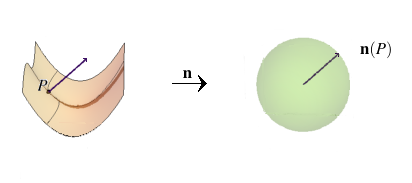
\includegraphics[scale=1.1]{mygauss}}
    \caption[The Gauss Map]{\label{fig:mygauss}
    The mapping of a point $P$ to $\vect{n}(P)$ by the Gauss map \cite{Rogers2011}}
\end{figure}

In order to understand how the surface is curving we will study how the unit normals change along the surface. We do this by slicing $M$ through a point $P$ by the plane spanned by $\vect{n}(P)$ and some unit vector $\vect V\,\in\,T_PM$. We then make use of the \textit{directional derivative} to see how the unit normal changes as we move in the direction of $\vect V$. 

Let $\alpha$ be the parametized curve formed by any normal slice with $\alpha(0)\,=\,P$ and $\alpha'(0)\,=\,\vect V$. We consider the curve $\vect n\circ \alpha(t)\,=\,\vect n(t)$ in $\Sigma$ (since it is the image under the gauss map). Hence we have restricted the unit normal to our curve $\alpha(t)$. Then the tangent vector $\vect{n}'(0)\,=\,D_{\vect V}\vect n(P)$ lies in $T_PM$. This vector measures the rate of change of $\vect n$ restricted to $\alpha(t)$, at $t\,=\,0$. Hence we have a measure of how $\vect n$ moves away from $\vect n(P)$ in a neighbourhood of $P$ \cite{Shifrin2016}.$\\$


\begin{remark}
The fact that $D_{\vect V}\vect n(P)$ lies in $T_PM$ will be shown in the proposition below. Here we introduce the concept of the \textit{shape operator}, it is simply the negative of the directional derivative at a point $P$ in the direction of some tangent vector. We note the negative sign in the definition, it may seem arbitrary for now but, as we shall see, introducing a negative here reduces the number of negatives later on.$\\$
\end{remark}

\begin{prop}
For any $ \vect{V}\,\in\,T_PM $, the directional derivative $D_{\vect{v}}\vect{n}(P)\,\in\,T_PM$. Moreover, the linear map $S_P\vcentcolon\,T_PM\,\to\,T_PM$ defined by
\begin{align*}
S_P(\vect{V})\,=\,-D_{\vect{V}}\vect{n}(P).
\end{align*}
is a symmetric linear map. That is, for any $\vect{U},\,\vect{V}\,\in\,\,T_PM$, we have
\begin{align*}
S_P(\vect{U})\cdot\vect{V}\,=\,\vect{U}\cdot S_P(\vect{V}).
\end{align*}
$S_P$ is called the \textit{shape operator} at $P$.
\end{prop}

\begin{proof}
For any curve $\vect{\alpha}\vcentcolon(-\epsilon,\,\epsilon)\,\to\,M$ with $\vect{\alpha}(0)\,=\,P$ and $\vect{\alpha}'(0)\,=\,\vect{V}$. Note that $\vect n\circ\vect{\alpha}$ has constant length 1 since
\begin{align*}
\vect n\cdot\alpha(0)\,=\,\vect{n}(\alpha(0))\,=\,\vect{n}(P).
\end{align*}
which, by definition, is a unit vector. Hence, by Lemma \ref{lemma:calc}, $D_\vect{V}\vect{n}(P)\cdot\vect{n}(P)\,=\,(\vect{n}\circ\vect{\alpha})'(0)\cdot(\vect{n}\circ\vect{\alpha})(0)\,=\,0$, so $D_\vect{V}\vect{n}(P)$ lies in the tangent plane to $M$ at $P$. $S_P$ is a linear map since $D_\vect V f(P)\,=\,\nabla f(P)\cdot\vect V$ which implies the directional derivative is a linear function of $\vect V$.

We first consider $\vect U\,=\,\vect{x}_u,\,\vect{V}\,=\,\vect{x}_v$. Note that $\vect{n}\cdot\vect{x}_v\,=\,0$, so $0\,=\,(\vect{n}\cdot\vect{x}_v)_u\,=\,\vect{n}_u\cdot\vect{x}_v\,+\,\vect{n}\cdot\vect{x}_{vu}$. Hence,
\begin{align*}
S_P(\vect x_u)\cdot\vect x_v\,=\,-D_{\vect{x}_u}\vect{n}(P)\cdot\vect x_v\,=\,-\vect{n}_u\cdot\vect{x}_v\,&=\,\vect{n}\cdot\vect{x}_{vu}\\
&=\,\vect{n}\cdot\vect{x}_{uv}\,=\,-\vect{n}_v\cdot\vect{x}_u\,=\,-D_{\vect{x}_v}\vect{n}(P)\cdot\vect x_u\,=\,S_P(\vect x_v)\cdot\vect x_u.
\end{align*}
Now consider $\vect{U}\,=\,a\vect x_u\,+\,b\vect x_v$ and $\vect{V}\,=\,c\vect x_u\,+\,d\vect x_v$, then
\begin{align*}
S_P(\vect{U})\cdot\vect V\,&=\,S_P(a\vect x_u\,+\,b\vect x_v)\cdot(c\vect x_u\,+\,d\vect x_v)\\
&=\,(aS_P(\vect x_u)\,+\,bS_P(\vect x_v))\cdot(c\vect x_u\,+\,d\vect x_v)\\
&=\,acS_P(\vect x_u)\cdot\vect x_u\,+\,adS_P(\vect x_u)\cdot\vect x_v\,+\,bcS_P(\vect x_v)\cdot\vect x_u\,+\,bdS_P(\vect x_v)\cdot\vect x_v\\
&=\,acS_P(\vect x_u)\cdot\vect x_u\,+\,adS_P(\vect x_v)\cdot\vect x_u\,+\,bcS_P(\vect x_u)\cdot\vect x_v\,+\,bdS_P(\vect x_v)\cdot\vect x_v\\
&=\,(a\vect x_u\,+\,b\vect x_v)\cdot(cS_P(\vect x_u)\,+\,dS_P(\vect x_v))\,=\,\vect U \cdot S_P(\vect V).
\end{align*}
as required.
\end{proof}

We now define the \textit{Second Fundamental Form} based on the results of the above.
\section{The Second Fundamental Form}
\begin{definition}{The Second Fundamental Form}
Let $M$ be a regular surface with $\vect{U},\,\vect{V}\,\in\,T_PM$. Then the \textit{Second Fundamental Form} is defined to be
\begin{align*}
\RN{2}_P(\vect{U},\vect{V})\,=\,S_P(\vect{U})\cdot\vect{V}.
\end{align*}
Since $M$ regular we again use the natural basis $\{\vect{x_{\bm{u}}},\vect{x_{\bm{v}}}\}$, and so we define
\begin{align*}
l\,&=\,\RN{2}_P(\vect x_u,\vect x_u)\,=\,-D_{\vect x_u}\vect n\cdot \vect x_u\,=\,\vect x_{uu}\cdot\vect n,\\
m\,&=\,\RN{2}_P(\vect x_u,\vect x_v)\,=\,-D_{\vect x_u}\vect n\cdot \vect x_v\,=\,\vect x_{vu}\cdot\vect n\,=\,\vect x_{uv}\cdot\vect n\,=\,\RN{2}_P(\vect x_v,\vect x_u),\\
n\,&=\,\RN{2}_P(\vect x_v,\vect x_v)\,=\,-D_{\vect x_v}\vect n\cdot \vect x_v\,=\,\vect x_{vv}\cdot\vect n.\\
\end{align*}
This is the reason we introduced a negative in the definition for the shape operator. So that the above three equations do not all require a negative on the outside.

Now if $\vect{U}\,=\,a\vect x_u\,+\,b\vect x_v$ and $\vect{V}\,=\,c\vect x_u\,+\,d\vect x_v$, then
\begin{align*}
\RN{2}_P(\vect U, \vect V)\,&=\,\RN{2}_P(a\vect x_u\,+\,b\vect x_v,\,c\vect x_u\,+\,d\vect x_v)\\
&=\,ac\RN{2}_P(\vect x_u,\,\vect x_u)\,+\,ad\RN{2}_P(\vect x_u,\,\vect x_v)\,+\,bc\RN{2}_P(\vect x_v,\,\vect x_u)\,+\,bd\RN{2}_P(\vect x_v,\,\vect x_v)\\
&=\,l(ac)\,+\,m(bc\,+\,ad)\,+\,n(bd).
\end{align*}
As it turns out, this too can be represented as a symmetric matrix, as follows
\begin{align*}
S_P(\vect U)\cdot\vect V\,&=\,S_P(a\vect x_u\,+\,b\vect x_v)\cdot[c\vect x_u\,+\,d\vect x_v]\\
&=\,
\begin{bmatrix}
    -aD_{\vect x_u}\vect n(P) \\
    -bD_{\vect x_v}\vect n(P)
\end{bmatrix}
\cdot [c\vect x_u\,+\,d\vect x_v]
\,=\,
\begin{bmatrix}
    -a\vect n_u\\
    -b\vect n_v
\end{bmatrix}
\cdot [c\vect x_u\,+\,d\vect x_v]\\
&=\,
\begin{bmatrix}
    -ac\vect n_u\vect x_u && -ad\vect n_u\vect x_v\\
    -bc\vect n_v\vect x_u && -bd\vect n_v\vect x_v
\end{bmatrix}
\,=\,
\begin{bmatrix}
    ac\vect x_{uu}\cdot\vect{n} && ad\vect{x}_{uv}\cdot\vect{n}\\
    bc\vect x_{vu}\cdot\vect{n} && bd\vect x_{vv}\cdot\vect{n}
\end{bmatrix}\\
&=\,
\begin{bmatrix}
a\\
b
\end{bmatrix}^\intercal
\begin{bmatrix}
l && m\\
m && n
\end{bmatrix}
\begin{bmatrix}
c\\
d
\end{bmatrix}.
\end{align*}
That is
\begin{align*}
\RN{2}_P(\vect U, \vect V)\,=\,
\begin{bmatrix}
l && m\\
m && n
\end{bmatrix}.
\end{align*}

Again if $\alpha$ is a parametized curve lying in $M$ with $\alpha(0)\,=\,P$ and $\alpha'(0)\,=\,\vect V$. Then since $(\vect n\circ\alpha(t))\cdot\alpha'(t)\,=\,0$ in a neighbourhood of $t$, applying Lemma \ref{lemma:calc} gives us that
\begin{align*}
(\vect n\circ\alpha)(t)\cdot\alpha''(t)\,=\,-(\vect n\circ\alpha)'(t)\cdot\alpha'(t).
\end{align*}
and so
\begin{align}
\RN{2}_P(\vect V, \vect V)\,=\,-D_{\vect V}\vect n(P)\cdot\vect V\,=\,-(\vect n\circ\alpha)'(0)\cdot\alpha'(0)\,=\,\vect n(P)\cdot\alpha''(0)\,=\,\kappa\vect N\cdot\vect n(P).\label{eq:RNtwo}\\\nonumber
\end{align}

\begin{remark}
When studying the differential geometry of curves through space we have that the \textit{principal normal vector} is defined as $\vect N\,=\,\dfrac{\vect V'}{\lvert \lvert \vect V' \rvert\rvert}$ and the \textit{curvature} is defined as $\kappa\,=\,\lvert\lvert\vect V'\rvert\rvert$. Then $\vect V'\,=\,\kappa\vect N$, hence the result in equation \ref{eq:RNtwo}.
\end{remark}
\end{definition}

\begin{definition}\label{def:normalcurv}
The component of the curvature vector $\kappa\vect N$ of $\alpha$ normal to the surface $M$ at $P$ is called the \textit{normal curvature}, denoted $\kappa_n$.
\end{definition}

\begin{remark}
With definition \ref{def:normalcurv} and equation \ref{eq:RNtwo}, we have an interpretation for the second fundamental form: The value of $\RN{2}_P(\vect V, \vect V)$ for some unit vector in the tangent plane is equal to the normal curvature of a regular curve passing through $P$ and tangent to $\vect V$ \cite{DC1976}. This shows that the normal curvature is dependent only upon the direction of $\alpha$ at $P$ and nothing more. We also note that $\kappa_n$ can be computed using the second fundamental form alone. The following result can then be deduced
\end{remark}
\begin{prop}{(Meusnier's Formula)}
Let $\alpha$ be a curve on $M$ passing through $P$ with unit tangent vector $\vect V$. Then
\begin{align*}
\RN{2}_P(\vect V, \vect V)\,=\,\kappa_n\,=\,\kappa\cos\theta.
\end{align*}
where $\theta$ is the angle between the principal normal, $\vect N$, of $\alpha$ and the surface normal, $\vect n$, at $P$.
\end{prop}

\begin{proof}
Let $P$ be a point on our surface $M$. We consider a normal slice $C_n$ and a plane slice $C$. Let the angle between $C_n$ and $C$ be $\theta$. The x and y axes lie in the tangent plane and we take the $x$-axis to be tangent to the curves $\alpha_n$ and $\alpha$ (Formed by the intersection of the $C_n$ and $C$ with $M$) at the origin. Let $Q$ be a point on curve $\alpha$ as shown in Figure \ref{fig:Meusnier} below. Its coordinates are $(x,\,y,\,f(x,y))$. The perpindicular distance from $Q$ to the $x$-axis is $h$. We see $h$ is a function of $x$ and $y$ since
\begin{align*}
h(x,y)\,=\,\dfrac{\lvert f(x,y)\rvert}{\cos\theta}.
\end{align*}

\begin{figure}[H]
    \centerline{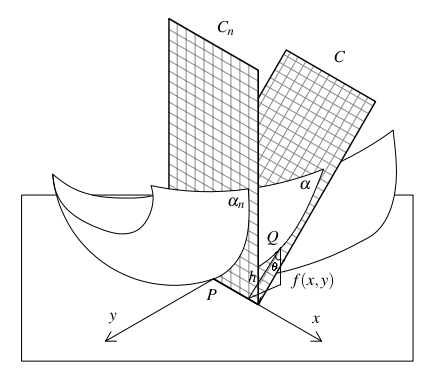
\includegraphics[scale=0.95]{Meusnier}}
    \caption[Meusnier's Theorem]{\label{fig:Meusnier}
    Meusnier's theorem construction, adapted from \cite{DC1976}}
\end{figure}

The curvature $\kappa$ of curve $\alpha$ is then, by Taylor's theorem, given by
\begin{align*}
\kappa\,&=\,\lim_{x\,\to\,0}\dfrac{2h(x,y)}{x^2}\,=\,\lim_{x\,\to\,0}2\dfrac{\lvert f(x,y)\rvert}{x^2\cos\theta}\\
&=\,\lim_{x\,\to\,0}\dfrac{f_{xx}x^2\,+\,2f_{xy}xy\,+\,f_{yy}y^2\,+\,2\epsilon}{x^2\cos\theta}.
\end{align*}
where $\epsilon\,\to\,0$ as $x,\,y\,\to\,0$. Since the $x$-axis is tangent to the curve $\alpha$, we have
\begin{align*}
\lim_{x\,\to\,0}\dfrac{y}{x}\,=\,0.
\end{align*}
Hence, taking the limit gives
\begin{align*}
\kappa\,=\,\dfrac{\lvert f_{xx}\rvert}{\cos\theta}.
\end{align*}
Now, for our chosen coordinate system, the curve $\alpha_N$ has the equation $z\,=\,f(x,\,0)$ and $\lvert\alpha_n\rvert\,=\,\lvert f_{xx} \rvert$. Thus
\begin{align*}
\kappa\,=\,\dfrac{\kappa_n}{\cos\theta}.
\end{align*}
\end{proof}

\begin{prop}
The matrix representing the linear map $S_P\vcentcolon\,T_PM\,\to\,T_PM$ with respect to basis $\{\vect{x_{\bm{u}}},\,\vect{x_{\bm{v}}}\}$ is
\begin{align*}
\RN{1}_P^{-1}\RN{2}_P\,=\,
\begin{bmatrix}
E && F\\
F && G
\end{bmatrix}^{-1}
\begin{bmatrix}
l && m\\
m && n
\end{bmatrix}.
\end{align*}
\end{prop}
\begin{proof}
Working in our basis $\{\vect x_u,\,\vect x_v\}$, we have
\begin{align*}
S_P(\vect x_u)\,=\,a\vect x_u\,+\,b\vect x_v\quad\text{and}\quad S_P(\vect x_v)\,=\,c\vect x_u\,+\,d\vect x_v.
\end{align*}
Then dotting each with $\vect x_u\,\,\text{and}\,\,\vect x_v$ gives
\begin{align*}
l\,=\,S_P(\vect x_u)\cdot\vect x_u\,=\,(a\vect x_u\,+\,b\vect x_v)\cdot\vect x_u\,=\,Ea\,+\,Fb,\\
m\,=\,S_P(\vect x_u)\cdot\vect x_v\,=\,(a\vect x_u\,+\,b\vect x_v)\cdot\vect x_v\,=\,Fa\,+\,Gb,\\
m\,=\,S_P(\vect x_v)\cdot\vect x_u\,=\,(a\vect x_u\,+\,b\vect x_v)\cdot\vect x_u\,=\,Ec\,+\,Fd,\\
n\,=\,S_P(\vect x_v)\cdot\vect x_v\,=\,(a\vect x_u\,+\,b\vect x_v)\cdot\vect x_u\,=\,Fc\,+\,Gd.\\
\end{align*}
putting this into a matrix gives
\begin{align*}
\begin{bmatrix}
l && m\\
m && n
\end{bmatrix}
\,&=\,
\begin{bmatrix}
Ea\,+\,Fb && Ec\,+\,Fd\\
Fa\,+\,Gb && Fc\,+\,Gd 
\end{bmatrix}\\\\
&=\,
\begin{bmatrix}
E && F\\
F && G
\end{bmatrix}
\begin{bmatrix}
a && c\\
b && d
\end{bmatrix}.
\end{align*}
so that
\begin{align*}
\begin{bmatrix}
a && c\\
b && d
\end{bmatrix}
\,=\,
\begin{bmatrix}
E && F\\
F && G
\end{bmatrix}^{-1}
\begin{bmatrix}
l && m\\
m && n
\end{bmatrix}
\,=\,\dfrac{1}{EG\,-\,F^2}
\begin{bmatrix}
G && -F\\
-F && E
\end{bmatrix}
\begin{bmatrix}
l && m\\
m && n
\end{bmatrix}
\,=\,\RN{1}_P^{-1}\RN{2}_P.
\end{align*}
as required.
\end{proof}
\begin{remark}
The matrix of the shape operator is not necessarily symmetric. However, if $\{\vect x_u,\vect x_v\}$ forms an orthonormal basis for $T_PM$ then we see that the matrix of the shape operator is simply the matrix of $\RN{2}_P$. Since if $\{\vect x_u,\vect x_v\}$ is orthonormal then we obviously have that
\begin{align*}
E\,=\,1\quad F\,=\,0 \quad G\,=\,1.
\end{align*}
We note that in this case 
\begin{align*}
\RN{1}_P^{-1}\,=\, \dfrac{1}{1}
\begin{bmatrix}
1 && 0\\
0 && 1
\end{bmatrix}.
\end{align*}
is simply the identity matrix. Hence the matrix of the shape operator is simply the matrix product of the identity with $\RN{2}_P$. Clearly in this case the matrix of the shape operator is symmetric.
\end{remark}

\section{The Extrinsic Properties}
We know from Linear Algebra that a symmetric $2\,\times\,2$ matrix has two real eigenvalues $\lambda_1$ and $\lambda_2$. Further, if $\lambda_1\,\neq\,\lambda_2$ then the corresponding eigenvector $\vect v_1$ and $\vect v_2$ are orthogonal. This leads us to define

\begin{definition}
The eigenvalues of $S_P$ are called the \textit{principal curvatures} of $M$ at $P$. Corresponding eigenvectors are called \textit{principal directions}. A curve in $M$ is called a \textit{line of curvature} if its tangent vector at each point is a principal direction. 
\end{definition}
If our principal directions are orthogonal then we may always choose an orthonomral basis for $T_PM$ consisting of the principal directions. Doing so allows us to easily calculate the curvature of any normal slice using the following

\begin{prop}\label{prop:407}
Let $\vect e_1,\, \vect e_2$ be unit vector in the principal directions at P with corresponding principal curvatures $\kappa_1$ and $\kappa_2$. Suppose $\vect V\,=\,\cos\theta\vect e_1\,=\,\sin\theta\vect e_2$ for some $\theta \,\in\,[0,2\pi)$, shown below. Then $\RN{2}_P(\vect V, \vect V)\,=\,\kappa_1\cos^2\theta \,+\,\kappa_2\sin^2\theta$.
\end{prop}
\begin{proof}
Since $S_P(\vect e_i)\,=\,\kappa_i\vect e_i$ for $i\,=\,1,2$ (As $e_i$ is an eigenvector of $S_P$), we have
\begin{align*}
\RN{2}_P(\vect V, \vect V)\,&=\,S_P(\vect V)\cdot\vect V\,=\,S_P(\cos\theta\vect e_1\,+\,\sin\theta\vect e_2)\cdot(\cos\theta\vect e_1\,+\,\sin\theta\vect e_2)\\
&=\,(\cos\theta \kappa_1\vect e_1\,+\,\sin\theta \kappa_2\vect e_2)\cdot(\cos\theta\vect e_1\,+\,\sin\theta\vect e_2)\\
&=\,\kappa_1\cos^2\theta\,+\,\kappa_2\sin^2\theta.
\end{align*}
as required.
\end{proof}

If we imagine a normal slice forming a straight line lying in our surface $M$, then clearly the curvature along this line is zero. This leads to another definiton

\begin{definition}
If the normal slice in direction $\vect V$ has zero curvature, that is if $\RN{2}_P(\vect V, \vect V)\,=\,0$, then $\vect V$ is an \textit{asymptotic direction}. A curve in $M$ is an \textit{asymptotic curve} if its tangent vector at each point is an asymptotic direction.
\end{definition}

A consequence of Proposition \ref{prop:407} is that the eigenvalues of $S_P$ are the maximum and minimum of the normal curvatures \cite{Shifrin2016}.

\begin{corol}
The principal curvatures are the maximum and minimum of the normal curvatures of the various normal slices.
\end{corol}

\begin{proof}
Assume that $\kappa_2\,\leq\,\kappa_1$. Then
\begin{align*}
\kappa_1\cos^2\theta\,+\,\kappa_2\sin^2\theta\,=\,\kappa_1(1\,-\,\sin^2\theta)\,+\,\kappa_2\sin^2\theta\,=\,\kappa_1\,+\,(\kappa_2\,-\,\kappa_1)\sin^2\theta\,\leq\,\kappa_1,
\end{align*}
and
\begin{align*}
\kappa_1\cos^2\theta\,+\,\kappa_2\sin^2\theta\,=\,\kappa_1\cos^2\theta\,+\,\kappa_2(1\,-\,\cos^2\theta)\,=\,(\kappa_1\,-\,\kappa_2)\cos^2\theta\,+\,\kappa_2\,\geq\,\kappa_2.
\end{align*}
and since $\RN{2}_P(\vect V,\vect V)\,=\kappa_1\cos^2\theta\,+\,\kappa_2\sin^2\theta\,=\,\kappa_n$, we have
\begin{align*}
\kappa_2\,\leq\,\kappa_n\,\leq\,\kappa_1.
\end{align*}
\end{proof}

\begin{definition}
The determinant of the shape operator, $S_P\vcentcolon\,T_PM\,\to\,T_PM$, is the \textit{Gaussian curvature} $K$ of $M$ at a point $P$. The half the trace of the shape operator is the \textit{mean curvature} $H$ of $M$ at $P$. That is
\begin{align*}
K\,&=\,\det S_P\,=\,\kappa_1\kappa_2,\\
H\,&=\,\dfrac{1}{2}\text{tr}\, S_P\,=\,\dfrac{1}{2}(\kappa_1\,+\,\kappa_2).
\end{align*}
\end{definition}

\begin{remark}
Recall from linear algebra that the determinant of a matrix is the product of it's eigenvalues, and the trace is the sum of the eigenvalues. Hence the above equations for $K$ and $H$. Further using the matrix of the shape operator above, we see
\begin{align*}
K\,=\,\det S_P\,&=\,\det\Bigg[\dfrac{1}{EG\,-\,F^2}
\begin{bmatrix}
G&&-F\\
-F&&E
\end{bmatrix}
\begin{bmatrix}
l&&m\\
m&&n
\end{bmatrix}\Bigg]\\
&=\,\dfrac{1}{\big(EG\,-\,F^2 \big)^2}\det
\begin{bmatrix}
Gl\,\-\,Fm&&Gm\,-\,Fn\\
Em\,-\,Fl&&En\,-\,Fm
\end{bmatrix}\\
&=\,\dfrac{1}{\big(EG\,-\,F^2 \big)^2}\Big((Gl\,-\,Fm)(En\,-\,Fm)\,-\,(Gm\,-\,Fn)(Em\,-\,Fl) \Big)\\
&=\,\dfrac{1}{\big(EG\,-\,F^2 \big)^2}\Big(EG(l\,-\,m^2)\,+\,FG(lm\,-\,lm)\,+\,EF(mn\,-\,mn)\,+\,F^2(ln\,-\,m^2)\Big)\\
&=\,\dfrac{(ln\,-\,m^2)(EG\,-\,F^2)}{(EG\,-\,F^2)^2}\\
&=\,
\dfrac{ln\,-\,m^2}{EG\,-\,F^2}.
\end{align*} 
\end{remark}

We now look at ways of classifying points on our surface based on the principal curvatures.

\begin{definition}
Let $P\,\in\,M$ be fixed. Then, $P$ is said to be
\begin{align*}
umbilic&\quad\text{if}\quad \kappa_1\,=\,\kappa_2,\\
planar&\quad\text{if}\quad \kappa_1\,=\,\kappa_2\,=\,0,\\
parabolic&\quad\text{if}\quad K\,=\,0,\,\,\text{but}\,\,P\,\,\text{is not planar},\\
elliptic&\quad\text{if}\quad K\,>\,0,\\
hyperbolic&\quad\text{if}\quad K\,<\,0.
\end{align*}
\end{definition}

\begin{example}
We return again to the torus from Example \ref{ex:232}. Using Figure \ref{fig:normaltorus} we can see that:

Taking normal slices on the outside of the torus, then any such slice would curve in the same direction (This should be obvious considering the parametization). Hence we have $K\,=\,\kappa_1\kappa_2\,>\,0$ and so the outside points are elliptic. Seen in the first figure.

Taking normal slices on the inside of the torus we see that along the horizontal line we have positive principal curvature and along the verical we have negative principal curvature. Hence $K\,=\,\kappa_1\kappa_2\,<\,0$ and so the inner most points are hyperbolic. Seen in the second figure.

Placing a tangent plane on top of the torus, if we take the normal lines along the curve of intersection, we see they remain constant. Hence for any point $P$ on this circle and $\vect V$ tangent, then $S_P(\vect V)\,=\,-D_{\vect V}\vect n\,=\,0$. Hence $\vect V$ is a principal direction with corresponding principal curvature 0 and so these are parabolic points. Seen in the last figure. 
\begin{figure}[H]
    \centerline{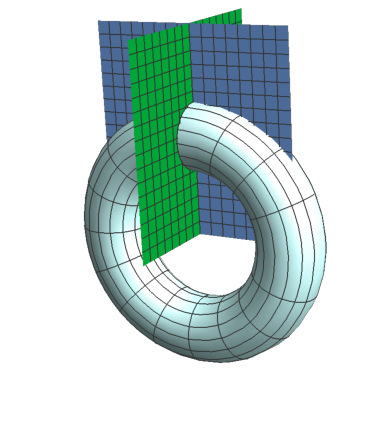
\includegraphics[scale=0.9]{outTorusSm}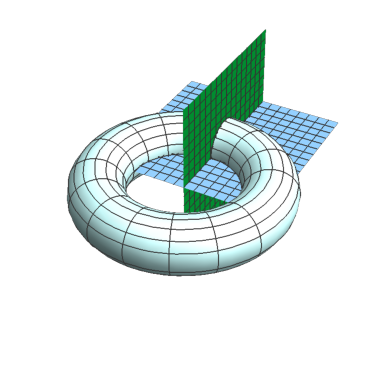
\includegraphics[scale=0.9]{innertorusSm}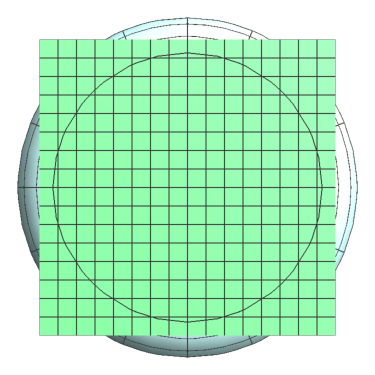
\includegraphics[scale=0.9]{toptorus}}
    \caption[Various Normal Slices on a Torus]{\label{fig:normaltorus}
    Various normal slices on a torus}
\end{figure}
\end{example}

\begin{example}
We once again return to the general surface of revolution. Recall
\begin{align*}
\vect x_u &= \big(f'(u)\cos v,\, f'(u)\sin v, \, g'(u)\big),\\
\vect x_v &= \big(-f(u)\sin v,\, f(u)\cos v, \,0\big),\\
\vect x_u\times \vect x_v &=\, f(u)\big(-g'(u)\cos v, \, -g'(u)\sin v,\, f'(u)\big).
\end{align*}
so we had
\begin{align*}
E\,=\,f'(u)^2\,+\,g'(u)^2\quad F\,=\,0\quad G\,=\,f(u)^2.
\end{align*}
and
\begin{align*}
\lvert\lvert\vect x_u \times \vect x_v\rvert\rvert\,=\,\lvert f(u)\rvert\sqrt{f'(u)^2\,+\,g'(u)^2}.
\end{align*}
from which we find
\begin{align*}
\vect n\,=\, \dfrac{\sgn(f)}{\sqrt{f'(u)^2\,+\,g'(u)^2}}(-g'(u)\cos v,-g'(u)\sin v,\,f'(u)).
\end{align*}

We now find the second order partial derivatives
\begin{align*}
\vect x_{uu} &=\,(f''(u)\cos v,\,f''(u)\sin v,\,g''(u)),\\
\vect x_{uv} &=\,(-f'(u)\sin v,\,f'(u)\cos v,\,0),\\
\vect x_{vv} &=\,(-f(u)\cos v,\,-f(u)\sin v,\,0).
\end{align*}

which allows us to find the coefficients of the Second fundamental form
\begin{align*}
l &=\,\dfrac{\sgn(f)}{\sqrt{f'(u)^2\,+\,g'(u)^2}}\Big(f''(u)\cos v,\,f''(u)\sin v,\,g''(u)\Big)\cdot\Big(-g'(u)\cos v,-g'(u)\sin v,\,f'(u)\Big)\\
&=\,\dfrac{\sgn(f)}{\sqrt{f'(u)^2\,+\,g'(u)^2}}\Big(-f''(u)g'(u)\cos^2v\,-\,f''(u)g'(u)\sin^2v\,+\,f'(u)g''(u)\Big)\\
&=\,\dfrac{\sgn(f)}{\sqrt{f'(u)^2\,+\,g'(u)^2}}\Big(f'(u)g''(u)\,-\,f''(u)g'(u)\Big).\\
\end{align*}
\begin{align*}
m&=\,\dfrac{\sgn(f)}{\sqrt{f'(u)^2\,+\,g'(u)^2}}\Big(-f'(u)\sin v,\,f'(u)\cos v,\,0\Big)\cdot\Big(-g'(u)\cos v,-g'(u)\sin v,\,f'(u)\Big)\\
&=\,\dfrac{\sgn(f)}{\sqrt{f'(u)^2\,+\,g'(u)^2}}\Big( f'(u)g'(u)\sin v\cos v\,-\,f'(u)g'(u)\sin v\cos v \Big)\\
&=\,0.\\
\end{align*}
\begin{align*}
n&=\,\dfrac{\sgn(f)}{\sqrt{f'(u)^2\,+\,g'(u)^2}}\Big(-f(u)\cos v,\,-f(u)\sin v,\,0 \Big)\cdot\Big(-g'(u)\cos v,-g'(u)\sin v,\,f'(u)\Big)\\
&=\,\dfrac{\sgn(f)}{\sqrt{f'(u)^2\,+\,g'(u)^2}}\Big( f(u)g'(u)\cos^2v\,+\,f(u)g'(u)\sin^2v \Big)\\
&=\,\dfrac{\sgn(f)f(u)g'(u)}{\sqrt{f'(u)^2\,+\,g'(u)^2}}\\
&=\,\dfrac{\lvert f(u) \rvert g'(u)}{\sqrt{f'(u)^2\,+\,g'(u)^2}}.\\
&\Big(\text{Since}\,\,\sgn(f)\,=\,\dfrac{\lvert f \rvert}{f}\,\,\text{by definition} \Big)
\end{align*}
We now seek to find the principal curvatures $\kappa_1$ and $\kappa_2$ by using the matrix of the shape operator (The parameters $u,\,v$ have been omitted for brevity)
\begin{align*}
S_P\,&=\, \dfrac{1}{EG\,-\,F^2}
\begin{bmatrix}
G && -F\\
-F && E
\end{bmatrix}
\begin{bmatrix}
l && m\\
m && n
\end{bmatrix}\\
&=\,\dfrac{1}{f^2\big(f'^2\,+\,g'^2\big)}
\begin{bmatrix}
f^2 && 0\\
0 && (f'^2\,+\,g'^2)
\end{bmatrix}
\begin{bmatrix}
\dfrac{\sgn(f)\big(f'g''\,-\,f''g'\big)}{\sqrt{f'^2\,+\,g'^2}} && 0\\
0 && \dfrac{\lvert f \rvert g'}{\sqrt{f'^2\,+\,g'^2}}
\end{bmatrix}\\\\
&=\,
\begin{bmatrix}
\dfrac{1}{(f'^2\,+\,g'^2)} && 0\\
0 && \dfrac{1}{f^2}
\end{bmatrix}
\begin{bmatrix}
\dfrac{\sgn(f)\big(f'g''\,-\,f''g'\big)}{\sqrt{f'^2\,+\,g'^2}} && 0\\
0 && \dfrac{\lvert f \rvert g'}{\sqrt{f'^2\,+\,g'^2}}
\end{bmatrix}\\\\
&=\,
\begin{bmatrix}
\dfrac{\sgn(f)\big(f'g''\,-\,f''g'\big)}{\sqrt{\big(f'^2\,+\,g'^2\big)^3}} && 0\\
0 && \dfrac{g'}{\lvert f \rvert\sqrt{f'^2\,+\,g'^2}}
\end{bmatrix}.\\
\end{align*}
Now we know that $\det S_P\,=\,K\,=\,\kappa_1\kappa_2$, but since $S_P$ is a diagonal matrix, the eigenvalues correspond to the diagonal entries. Hence our principal curvatures are
\begin{align*}
\kappa_1\,=\,\dfrac{\sgn(f)\big(f'(u)g''(u)\,-\,f''(u)g'(u)\big)}{\sqrt{\big(f'(u)^2\,+\,g'(u)^2\big)^3}}\quad\text{and}\quad
\kappa_2\,=\,\dfrac{g'(u)}{\lvert f(u) \rvert\sqrt{f'(u)^2\,+\,g'(u)^2}}.
\end{align*}

Then using our definitions for the Gaussian and mean curvature we find

\begin{align*}
K\,=\,\kappa_1\kappa_2\,&=\, \dfrac{\sgn(f)\big(f'(u)g''(u)-f''(u)g'(u)\big)}{\sqrt{\big(f'(u)^2\,+\,g'(u)^2\big)^3}}\cdot\dfrac{g'(u)}{\lvert f(u) \rvert\sqrt{f'(u)^2\,+\,g'(u)^2}}\\\\
&=\,\dfrac{f'(u)g'(u)g''(u)\,-\,f''(u)g'(u)^2}{f(u)\big(f'(u)^2\,+\,g'(u)^2\big)^2}.\\\\
\end{align*}
\begin{align*}
H\,=\,\dfrac{1}{2}(\kappa_1\,+\,\kappa_2)\,&=\,\dfrac{1}{2}\bigg[\dfrac{\sgn (f)f(u)\big(f'(u)g''(u)\,-\,f''(u)g'(u)\big)\,+\,g'(u)\big(f'(u)^2\,+\,g'(u)^2\big)}{f(u)\sqrt{\big(f'(u)^2\,+\,g'(u)^2\big)^3}} \bigg]\\\\
&=\,\dfrac{f(u)\big(f'(u)g''(u)\,-\,f''(u)g'(u)\big)\,+\,g'(u)\big(f'(u)^2\,+\,g'(u)^2\big)}{2\lvert f(u) \rvert\sqrt{\big(f'(u)^2\,+\,g'(u)^2\big)^3} }.\\
\end{align*}
\end{example}

We make use of the following proposition to find the lines of curvature on the general surface of revolution

\begin{prop}
If $F\,=\,m\,=\,0$ then the parameter curves are lines of curvature.
\end{prop}

\begin{proof}
Suppose that $F\,=\,m\,=\,0$. Let $S_P(\vect x_u)\,=\,a\vect x_u\,+\,b\vect x_v$ and $S_P(\vect x_v)\,=\,c\vect x_u\,+\,d\vect x_v$. Then
\begin{align*}
0\,=\,S_P(\vect x_u)\cdot\vect x_v\,=\,aF\,+\,bG\,=\,bG.
\end{align*}
and
\begin{align*}
0\,=\,S_P(\vect x_v)\cdot\vect x_u\,=\,cE\,+\,dF\,=\,cE.
\end{align*}
and so we have that $b\,=\,c\,=\,0$. This implies that $\vect x_u$ and $\vect x_v$ are eigenvectors of $S_P$. Hence the parameter curves are lines of curvature. 
\end{proof}

\begin{remark}
The above proposition tells us that the parallels and meridians of the general surface of revolution constitute the lines of curvature. That is, $u\,=$ const and $v\,=$ const, are the lines of curvature.
\end{remark}

We close off by looking at Gauss's \textit{Theorema Egregium}, which means the "Remarkable Theorem". It states that the Gaussian curvature of a surface is an intrinsic property. This indeed is remarkable as our definition for the Gaussian curvature was the determinant of the shape operator, but this requires reference to the embedding of the surface. We first need a lemma to aid us in the proof.

\begin{lemma}\label{lem:1}
Let $(\vect e,\,\vect f,\, \vect n)$ be an orthonormal triple of vector fields on a surface $M$ with parametization $\vect x(u,v)$, where $\vect n$ is the unit normal to the surface. Then
\begin{align*}
\vect e_u\cdot \vect f_v\,-\, \vect e_v\cdot\vect f_u\,=\,\dfrac{ln\,-\,m^2}{\sqrt{EG\,-\,F^2}}.
\end{align*}
\end{lemma}

\begin{proof}
It can be shown that $\vect n_u\,\times\,\vect n_v\,=\,K(\vect x_u\,\times\,\vect x_v)$. Therefore
\begin{align*}
(\vect n_u\,\times\,\vect n_v)\cdot\vect n\,=\,K(\vect x_u\,\times\,\vect x_v)\cdot\vect n\,=\,K\lvert \vect x_u\,\times\,\vect x_v\rvert\vect n\cdot \vect n\,=\,\dfrac{ln\,-\,m^2}{\sqrt{EG\,-\,F^2}}.
\end{align*}
by the above remark on a formula for $K$ and that $\lvert\lvert\vect x_u\,\times\,\vect x_v\rvert\rvert\,=\,\sqrt{EG\,-\,F^2}$. Now
\begin{align*}
(\vect n_u\,\times\,\vect n_v)\cdot\vect n\,=\,(\vect n_u\,\times\,\vect n_v)\cdot(\vect e\,\times\,\vect f)\,=\,(\vect n_u\cdot\vect e)(\vect n_v\cdot\vect f)\,-\,(\vect n_v\cdot\vect e)(\vect n_u\cdot\vect f).
\end{align*}
Furthermore
\begin{align*}
\vect n\cdot\vect e \,\equiv\quad\Longrightarrow\quad 0\,\equiv\,(\vect n\cdot\vect e)_u\,=\,\vect n_u\cdot\vect e\,+\,\vect n\cdot\vect e_u\quad\Longrightarrow\quad\vect n_u\cdot\vect e\,=\,-\vect n\cdot\vect e_u.
\end{align*}
and simly $\vect n_v\cdot\vect e\,=\,-\vect n\cdot\vect e_v$. The same holds when $\vect e$ is replaced with $\vect f$. Hence
\begin{align*}
\dfrac{ln\,-\,m^2}{\sqrt{EG\,-\,F^2}}\,=\,(\vect n\cdot\vect e_u)(\vect n\cdot\vect f_v)\,-\,(\vect n\cdot\vect e_v)(\vect n\cdot\vect f_u).
\end{align*}
Finally, when writing $\vect e_u,\,\vect e_v,\,\vect f_u\,\,\text{and}\,\,\vect f_v$ in terms of the orthonormal basis $\{\vect e,\,\vect f,\,\vect n\}$ certain terms will not appear since $\vect e\cdot\vect e\,=\,1$ and so $\vect e\cdot\vect e_u\,=\,0\,=\,\vect e\cdot\vect e_v$. Similarily for $\vect f$. Hence
\begin{align*}
\vect e_u\,&=(\vect f\cdot\vect e_u)\vect f\,+\,(\vect n\cdot\vect e_u)\vect n,\\
\vect e_v\,&=(\vect f\cdot\vect e_v)\vect f\,+\,(\vect n\cdot\vect e_v)\vect n,\\
\vect f_u\,&=(\vect e\cdot\vect f_u)\vect e\,+\,(\vect n\cdot\vect f_u)\vect n,\\
\vect f_v\,&=(\vect e\cdot\vect f_v)\vect e\,+\,(\vect n\cdot\vect f_v)\vect n.
\end{align*}
and so
\begin{align*}
\vect e_u\cdot\vect f_v\,-\,\vect e_v\cdot\vect f_u\,=\,(\vect n\cdot\vect e_u)(\vect n\cdot\vect f_v)\,-\,(\vect n\cdot\vect e_v)(\vect n\cdot\vect f_u)\,=\,\dfrac{ln\,-\,m^2}{\sqrt{EG\,-\,F^2}}.
\end{align*}
\end{proof}

We are now in a suitable position to prove Gauss's \textit{Theorema Egregium}.

\begin{theorem}{(Theorema Egregium)}
Let $\vect x\vcentcolon\,U\,\to\,M$ and $\vect x^*\vcentcolon\,U\,\to\,M^*$ be parametizations of surfaces $M$ and $M^*$ respectively. If these surfaces are isometric, then their Gaussian curvatures are equal.
\end{theorem}

\begin{proof}
From Lemma \ref{lem:1} we have that
\begin{align*}
K\,=\,\dfrac{\vect e_u\cdot\vect f_v\,-\,\vect e_v\cdot\vect f_u}{\sqrt{EG\,-\,F^2}}.
\end{align*}
Hence we need only show that $\vect e_u\cdot\vect f_v\,-\,\vect e_v\cdot\vect f_u$ depends only on the coefficients of the first fundamental form and their partial derivatives, when $\vect e$ and $\vect f$ are suitably chosen. Let
\begin{align*}
\vect e\vcentcolon=\,\dfrac{\vect x_u}{\lvert\vect x_u\rvert}\quad\text{and}\quad\vect f\vcentcolon = \,\dfrac{\vect x_v\,-(\vect e\cdot\vect x_v)\vect e}{\lvert \vect x_v\,-(\vect e\cdot\vect x_v)\vect e\rvert}.
\end{align*}
since $\{\vect x_u,\,\vect x_v\}$ is linearly independent everywhere, the vector fields $\vect e$ and $\vect f$ are well defined. By construction, $\{\vect e,\,\vect f,\,\vect n\}$ is an othonormal basis everywhere. Now,
\begin{align*}
\deriv{}{v}(\vect e_u\cdot\vect f)\,-\,\deriv{}{u}(\vect e_v\cdot\vect f)\,&=\,\vect e_{vu}\cdot\vect f\,+\,\vect e_u\cdot\vect f_v\,-\vect e_{uv}\cdot\vect f\,-\,\vect e_v\cdot\vect f_u\\
&=\vect e_u\cdot\vect f_v\,-\,\vect e_v\cdot\vect f_u,\\\\
\lvert\vect x_u\rvert\,&=\,E^{1/2},\\\\
\text{and}\quad\lvert\vect x_v\,-\,(\vect e\cdot\vect x_v)\vect e\rvert\,&=\,\lvert \vect x_u\,-\,\lvert\vect x_u\rvert^{-2}(\vect x_u\cdot\vect x_v)\vect x_u \rvert\\
&=\,\lvert \vect x_v\,-\,E^{-1}F\vect x_u \rvert \\
&=\,(G\,-\,2E^{-1}F^2\,+\,E^{-2}F^2E)^{1/2}\\
&=\,E^{-1/2}(EG\,-\,F^2)^{1/2}.
\end{align*}
and since
\begin{align*}
E_u\,&=\,2\vect x_u\cdot\vect x_{uu} &E_v\,&=\,2\vect x_u\cdot\vect x_{uv},\\
F_u\,&=\,\vect x_u\cdot\vect x_{uv}\,+\,\vect x_v\vect x_{uu} &F_v\,&=\,\vect x_u\cdot\vect x_{vv}\,+\,\vect x_v\cdot\vect x_{uv},\\
G_u\,&=\,2\vect x_v\cdot\vect x_{uv} &G_v\,&=\,2\vect x_v\cdot\vect x_{vv}.
\end{align*}
we can now find
\begin{align*}
\vect e_u\cdot\vect f\,&=\,\Bigg(\dfrac{E_u\vect x_u}{2E^{3/2}}\,+\,\dfrac{\vect x_{uu}}{E^{1/2}}\Bigg)\cdot\dfrac{E^{1/2}(\vect x_v\,-\,E^{-1}F\vect x_u}{(EG\,-\,F^2)^{1/2}}\\
&=\,\dfrac{\vect x_{uu}\cdot\vect x_v}{(EG\,-\,F^2)^{1/2}}\,-\,\dfrac{F\vect x_{uu}\cdot\vect x_u}{E(EG\,-\,F^2)^{1/2}}\,=\,\dfrac{2F_u\,-\,E_v}{2(EG\,-\,F^2)^{1/2}}\,-\,\dfrac{FE_u}{2E(EG\,-\,F^2)^{1/2}},\\
\vect e_v\cdot\vect f\,&=\,\Bigg(\dfrac{E_V\vect x_u}{2E^{3/2}}\,+\,\dfrac{\vect x_{vu}}{E^{1/2}}\Bigg)\cdot\dfrac{E^{1/2}(\vect x_v\,-\,E^{-1}F\vect x_u}{(EG\,-\,F^2)^{1/2}}\\
&=\,\dfrac{\vect x_{vu}\cdot\vect x_u}{(EG\,-\,F^2)^{1/2}}\,-\,\dfrac{F\vect x_{vu}\cdot\vect x_u}{E(EG\,-\,F^2)^{1/2}}\,=\,\dfrac{G_u}{2(EG\,-\,F^2)^{1/2}}\,-\,\dfrac{FE_v}{2E(EG\,-\,F^2)^{1/2}}.\\
\end{align*}

and so $\,\vect e_u\cdot\vect f_v\,-\,\vect e_v\cdot\vect f_u\,$ depends only on $E,\,F,$ and $G$ and their partial derivatives. That is, the Gaussian curvature can be calculated using the First Fundamental form alone.
\end{proof}

\begin{remark}
This result leads to an interesting way of answering whether or not there exists an isometric mapping between two surfaces. If our two surfaces have different Gaussian Curvature (which is invarient under reparametisation), then no isometric map can exist between our two surfaces, regardless of how we try and parametise them \cite{DC1976}. A great example of this is the sphere and the plane, since their Gaussian curvatures are different, no isometric map exists between them. Hence there is no stereographic projection of the earth onto a flat map which preserves distances. 
\end{remark}
\chapter{Conclusion}

We have seen the First and Second Fundamental form fully capture the metric properties of the surface and key relationships exists between a geometric object it's partial derivatives. The First Fundamental form allows intrinsic questions to be adequately treated, whereas the second fundamental form caters for extrinsic questions. As one would hope, we found that these results are independent of the parametization chosen. A surprising result was found regarding the Gaussian curvature and it's direct relation to the first fundamental form, giving a new way to determine whether surfaces are locally isometric.  These ideas can be extended to higher dimensions to study manifolds (n-dimensional spaces which locally resembles Euclidean space at each point) and other interesting concepts such as the contact geometry.

 % Make the bibliography.

 %\clearpage

 \bibliography{references}
 

 % Make the index
 \cleardoublepage
 \singlespace
 % NOTE: '\phantomsection' helps get the pdf bookmark to work right. You need
 % to put it before every manual addition to the table of contents
 \phantomsection
 \addcontentsline{toc}{chapter}{Index}
 \printindex

\end{document}
